% options:
% thesis=B bachelor's thesis
% thesis=M master's thesis
% czech thesis in Czech language
% slovak thesis in Slovak language
% english thesis in English language
% hidelinks remove colour boxes around hyperlinks


\documentclass[thesis=B,czech]{FITthesis}[2012/06/26]

\usepackage[utf8]{inputenc} % LaTeX source encoded as UTF-8

\usepackage{color}
\definecolor{light-gray}{gray}{0.95}

\usepackage{listings} % source codes
\renewcommand{\lstlistingname}{Zdrojový kód}
\renewcommand{\lstlistlistingname}{Seznam ukázek kódu}

\lstset{
  captionpos=b,                           % sets the caption-position to top
  abovecaptionskip=12pt,
  backgroundcolor = \color{light-gray},
  basicstyle=\ttfamily,breaklines=true
 }

\usepackage{graphicx} %graphics files inclusion
% \usepackage{amsmath} %advanced maths
% \usepackage{amssymb} %additional math symbols

\usepackage{dirtree} %directory tree visualisation

\usepackage[table,xcdraw]{xcolor}

\lstdefinelanguage{json}{
	showstringspaces=false,
	numbers=left,
	breaklines=true
	tabsize=2,
}




% % list of acronyms
% \usepackage[acronym,nonumberlist,toc,numberedsection=autolabel]{glossaries}
% \iflanguage{czech}{\renewcommand*{\acronymname}{Seznam pou{\v z}it{\' y}ch zkratek}}{}
% \makeglossaries

\newcommand{\tg}{\mathop{\mathrm{tg}}} %cesky tangens
\newcommand{\cotg}{\mathop{\mathrm{cotg}}} %cesky cotangens

% % % % % % % % % % % % % % % % % % % % % % % % % % % % % % 
% ODTUD DAL VSE ZMENTE
% % % % % % % % % % % % % % % % % % % % % % % % % % % % % % 

\department{Katedra softwarového inženýrství}
\title{Systém pro analýzu proudu dat v reálném čase}
\authorGN{David} %(křestní) jméno (jména) autora
\authorFN{Viktora} %příjmení autora
\authorWithDegrees{David Viktora} %jméno autora včetně současných akademických titulů
\supervisor{Ing. Adam Šenk}
\acknowledgements{Poděkování ....}
\abstractCS{Cílem této práce bylo vytvoření systému pro analýzu proudu dat v reálném čase v kontextu velkých objemů dat. Zpracovávanými daty jsou příspěvky ze sociální sítě Twitter. K samotné analýze byl použit framework Apache Spark, výsledky z něj jsou ukládány do klasické relační databáze a zpřístupněné pomocí REST API. Vytvořený systém umožňuje monitorovat přání uživatelů Twitteru. Díky analýze sentimentu těchto příspěvků by po drobných úpravách mohl být vyvinutý systém použit například při provádění předvolebních průzkumů či analýze oblíbenosti produktů vybrané společnosti. }
\abstractEN{Sem doplňte ekvivalent abstraktu Vaší práce v~angličtině.}
\placeForDeclarationOfAuthenticity{V~Praze}
\declarationOfAuthenticityOption{4} %volba Prohlášení (číslo 1-6)
\keywordsCS{Apache Spark, proudové zpracování dat, Big Data, Twitter, sentimentální analýza, REST API}
\keywordsEN{Nahraďte seznamem klíčových slov v angličtině oddělených čárkou.}


\begin{document}

% \newacronym{CVUT}{{\v C}VUT}{{\v C}esk{\' e} vysok{\' e} u{\v c}en{\' i} technick{\' e} v Praze}
% \newacronym{FIT}{FIT}{Fakulta informa{\v c}n{\' i}ch technologi{\' i}}

\lstlistoflistings

\begin{introduction}
	V současné době generujeme obrovská množství dat - podle některých odhadů to například v roce 2012 mohlo být až 2,5 exabajtů za den\cite{bbc-bigdata}, od té doby se rychlost jejich přibývání stále zvyšuje. Spolu s nárůstem objemu dat je potřeba vyvinout nové metody umožňující jejich zpracování v přijatelném čase. 
	
	Cílem této práce je pomocí frameworku Apache Spark vyvinout systém pro analýzů příspěvků ze sociální sítě Twitter. Tato analýza probíhá v reálném čase a umožňuje monitorovat příspěvky reprezentující přání jejich autorů. U těchto přání je prováděna mimo jiné analýza sentimentu jejímž výsledkem je hodnocení pozitivity daného příspěvku. Výsledky této analýzy jsou ukládány do relační databáze a zpřístupněny pomocí REST API. Pro prezentaci výsledků byla vytvořena také webová stránka. 
	
	Text této práce je členěn šesti kapitol. V první kapitole se věnuji současné situaci v oblati zpracování dat. Zaměřuji se na vysvětlení některých pojmů a zabývám se také dostupnými technologiemi umožňujícími zpracování velkých objemů dat. Druhá kapitola pak obsahuje informace o nejrozšířenějších metodách analýzy textu a o sociální síti Twitter. Jsou v ní také definovány požadavky pro vyvinutý systém. 
	
	V třetí kapitole nejprvne obecně analyzuji jednotlivé komponenty systému, abych posléze podrobněji popsal jejich implementaci a k tomu použité konkrétní technologie v kapitole \ref{implementace}. Pátá kapitola se věnuje testování implementovaného systému a v poslední kapitole jsou shrnuty dosažené výsledky a přínosy této práce. 
	
\end{introduction}

%\chapter
%\section
%\subsection
%


\chapter{Situace v oblasti zpracovávání dat}
	Například nárůst objemu dat dostupných na internetu je způsoben jeho neustále větším rozšířením a rostoucí dostupností. V  roce 2016 je k němu připojeno již přes 3,3 miliardy obyvatel planety\cite{internet-live-stats}, což je téměř polovina celkové populace. Roste také míra využívání internetu. Oproti dřívějšku na internetu trávíme nejen díky chytrým telefonům stále více času a využíváme například sociální sítě, internetové vyhledávání a další online služby. Během toho jsou nám zobrazována personalizovaná data a cílené reklamní nabídky. Také ve firemní i státní sféře výrazně roste stupeň využívání informačních technologií a v návaznosti na to objem produkovaných dat. S přibývajícími daty nastávají problémy s jejich zpracováním. Jedním z nich je obecně schopnost zpracovat tak veliké objemy dat, druhým je schopnost jejich zpracování v dostatečně krátkém, ideálně reálném čase. Často je přitom potřeba vyřešit oba tyto problémy naráz. Pro popis těchto dat a problémů spojených s jejich zpracováním se používá relativně nový pojem Big Data. 

		 
\section{Big Data a technologie pro práci s nimi}
	Právě pojem Big Data je často označován za jeden z největších buzzwords\footnote{Slova nebo fráze, které jsou v současné době populární} současného IT světa. I přes jeho popularitu nejsou přesně vymezené jeho hranice či definované pojmy zabývající se toutu oblastí. Obecně můžeme říci, že o Big Datech hovoříme v případech, kdy je potřeba zpracovávat objemy dat v řádech gigabajtů a více. To je velice zjednodušený popis tohoto termínu, přesná definice však neexistuje a na celý problém se dá dívat různými způsoby. Rozšířené je například také tvrzení říkající, že o Big Datech mluvíme zkrátka v těch případech, kdy klasické databázové a softwarové nástroje především kvůli objemu těchto dat selhávají\cite{webopedia-bigdata}. 

	Přestože jednotná definice neexistuje, ustálilo se několik problémů, kterým je při práci s Big Daty potřeba čelit. Jedná se o takzvaná 3+1V - Volume, Velocity, Variety a později přidaná vlastnost Veracity\cite{dp-customer-inteligence}. Volume popisuje objem zpracovávaných dat, Velocity pak rychlost, jakou data přibývají. Charakteristikou Variety popisujeme různorodost dat a Veracity určuje úplnost a míru důvěryhodnosti dat. Ne vždy se setkáme se všemi těmito problémy naráz, každá z nich ale přidává na složitosti zpracování těchto dat. 
	
	Právě kvůli těmto vlastnostem se při práci s velkými objemy dat klasické technologie používané v minulosti stále častěji ukazují jako nedostatečně rychlé nebo obecně neschopné tato data zpracovat. Je proto nutné sáhnout po nových technologiích určených pro práci s nimi. Bez technologií pro Big Data se v dnešní době neobejdou třeba již zmiňované internetové vyhledávače nebo sociální sítě, využití ale nacházejí i v mnoha dalších oblastech. Jejich rozvoj je také předpokladem například pro další rozšíření tzv. Internet of Things\cite{bigdata-iot}.  

\subsection{Strukturovaná a nestrukturovaná data}	
	Data obecně často rozdělujeme do dvou kategorií - na data strukturovaná a nestrukturovaná. Strukturovaná data jsou obvykle uložena v klasické relační databázi, nebo obecně utříděna po řádcích a s přesně definovanými sloupci. Ostatní data, která nemají takto pevně danou strukturu, jsou data nestrukturovaná. Ještě donedávna docházelo ke zpracování téměř váhradně dat strukturovaných. Ta nestrukturovaná však často nabízejí obrovský potenciál k jejich využití. Klasickým příkladem nestrukturovaných dat je lidská řeč v psané formě - ta rozhodně obsahuje spoustu informací, ale ve formě kterou je počítačově složité analyzovat. Může se jednat například o články, konverzace nebo příspěvky na sociálních sítích.  Právě příspěvkům na sociální síti Twitter se věnuje i tato práce. 
	
	Analýzou lidské řeči se zabývá obor zvaný Natural Language Processing či Text Mining, obecně vytěžováním znalostí z dat pak tzv. Data Mining. Často skloňovaným pojmem je také Machine Learning, v češtině strojové učení. Pro všechny tyto obory jsou technologie pro Big Data obrovským přínosem - díky nim je možné získat opravdu cenné informace snáze a rychleji než bylo možné dříve. Například analýzou dat pohybu uživatele po webové stránce a jeho chováním můžeme odhalit nedostatky tohoto webu a jejich odstraněním zvýšit míru konverze. Hovoříme-li v kontextu sociální sítě Twitter, možnosti jsou ještě zajímavější. Na základě příspěvků a vyplněných informací jednotlivých uživatelů můžeme například odhadovat jejich volební preference nebo nabízet velice přesně cílenou reklamu. Konkrétnějším příkladem může být zajímavý projekt ze Stanfordské univerzity usilující o odhad vývoje cen akcií na základě analýzy sentimentu příspěvků z Twitteru\cite{stock-stanford}. Obecně metodám Text Miningu a především právě analýze sentimentu se věnuji v kapitole \ref{text-mining}.  

	Technologie pro Big Data je samozřejmě možné použít i na data strukturovaná, největší využití však nabízejí při zpracování těch nestrukturovaných. Protože nestruktorovaná data přibývají výrazně rychleji\cite{structured-unstructured}, a protože je jejich zpracování obvykle výpočetně náročnější, jsou právě technologie pro Big Data vhodnou volbou. 
 
	
\subsection{Principy zpracování velkých dat}
	Jedny z prvních konkrétních technologií pro práci s Big Daty vznikaly na přelomu tisíciletí ve společnosti Google. Právě Google v roce 2004 zveřejnil článek o modelu MapReduce\cite{mapreduce-google}, která se stala stavebním kamenem pro většinu dalších technologií pro práci s velkými objemy dat. MapReduce vlastně popisuje dvě nezávislé funkce. První z nich je funkce Map, ve které jsou ze vstupních dat vygenerovány dvojice klíč a hodnota. Poté co je funkce Map dokončena, její výstup je použit jako vstup do funkce Reduce. Ta pak spojí vstupní data podle klíče\cite{mapreduce-description}. 
	
	Klíčovou vlastností MapReduce modelu je možnost paralelizace Map fáze na počítačovém clusteru. Jeden z počítačů v clusteru například přijme požadavek od uživatele. Tento počítač rozdělí vstupní data ostatním počítačům v clusteru a vyčká na provedení Map fáze těmito počítači. Výsledná data pak sám master spojí v Reduce fázi a navrátí výsledek uživateli. Distribuce co největšího množství operací a výpočtů po počítačovém clusteru je v dnešní době obecně hlavním principem fungování technologií pro zpracování velkých objemů dat. Paradoxně nemusí jít o dražší řešení než nákup jednoho supervýkoného serveru. Clustery pro práci s Big Daty jsou totiž obvykle tvořeny běžně dostupnými a relativně levnými servery. 
	
	\begin{figure}[ht]
    	\centering
    	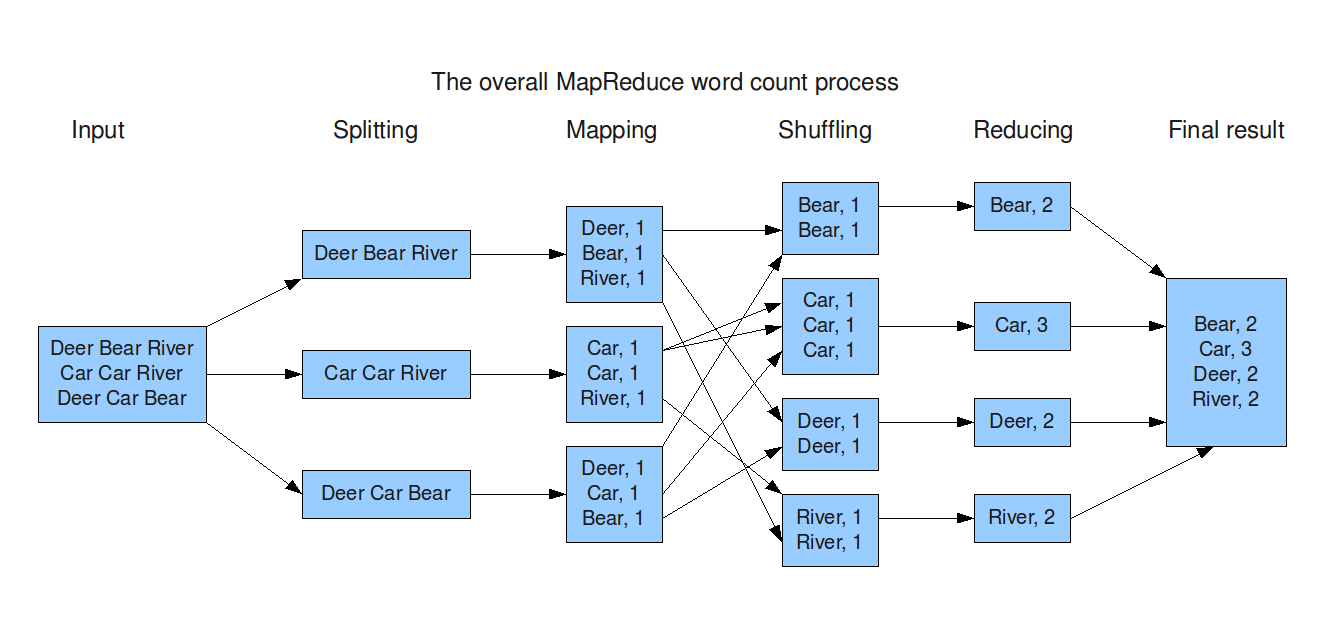
\includegraphics[width=1\textwidth]{images/mapreduce.png}
    	\caption{Ukázka fungování MapReduce paradigmatu \cite{mapreduce-img} }
    	\label{fig:mapreduce}
	\end{figure}
	
	Především v posledních letech se objevují konkrétní komplexnější nástroje pro práci s velkými daty. Tyto nástroje obvykle obsahují i další technologie, mimo jiné umožňující například správu a konzistenci počítačového clusteru. Tyto frameworky principielně data zpracovávají dvěma různými způsoby - jde o tzv. batchové zpracování nebo o zpracování streamové. 
	
\subsection{Batchové zpracování Big dat}
	Batchové neboli dávkové zpracování je vhodné především pro takové úkoly, jejichž výsledky není nutné znát ihned. Data jsou nejprve po určitou dobu shromažďována a až poté je jednorázově spuštěna úloha pro jejich zpracování. Toto zpracování obvykle zabere relativně dlouhý čas. Zmiňovaný MapReduce se využívá právě pro batchové zpracování dat. 

	Jedním z prvních klíčových frameworků který umožnil další vývoj v oblasti Big dat je jednoznačně open-source framework Hadoop\cite{hadoop-home}. Protože využívá MapReduce model podporuje právě batchové zpracování dat. Jeho první plná verze vyšla na konci roku 2011, ale byl využíván již přibližně od roku 2006 například ve společnosti Yahoo\cite{hadoop-history}. Je určen pro použití na počítačových clusterech složených z řádově desítek až stovek běžně dostupných serverů. Hadoop se skládá ze tří hlavních komponent - Hadoop Distributed File System, Hadoop MapReduce a Hadoop YARN. HDFS neboli Hadoop Distributed File System je distribuovaný filesystem zajišťující rozprostření dat po jednotlivých počítačích v clusteru. Klade důraz na toleranci výpadků částí clusteru. Pro zabránění ztráty dat v případě takového výpadku dochází mimo jiné k jejich replikaci na více strojů. Hadoop MapReduce je konkrétní implementace MapReduce modelu zmiňovaného dříve. Hadoop YARN pak slouží především k řízení zdrojů v clusteru, tedy například rozdělování práce jednotlivým serverům v clusteru. Nevýhodou Hadoopu je fakt, že nepodporuje proudové zpracování dat, ale pouze zpracování batchové. 
	
	V současné době jsou k dispozici i další batchově zaměřené frameworky, které často dosahují lepších výsledků než Hadoop a mimojiné obvykle umožňují vytváření úloh na vyšší úrovni. Díky ním například není nutné přímo vytvářet mapovací a reduce funkci. Nejrozšířenějím je bezesporu Apache Spark\cite{spark-home}, kterému se budu podrobněji věnovat v následujících sekcích. Oproti Hadoopu dosahuje především díky cachování a dalším vylepšením často několikanásobně kratší doby zpracování. Krom batchového zpracování umožňuje i práci s proudy dat. 

\subsection{Streamové zpracování}
	V praxi často potřebujeme velké objemy dat zpracovávat v co nejkratším čase a ideálně na každý nový podnět co nejdříve zareagovat. Batchové zpracování je v takovém případě nevhodné. Řešením je již zmiňované streamové zpracování, nebo také zpracování proudů dat. Vstupem do takového programu není fixní soubor dat, ale neustálý proud dat nových. Kdykoli program obdrží nový datový objekt, zjednodušeně ho začne okamžitě zpracovávat a mezivýsledky předávat mezi jednotlivými částmi programu nezávisle na dalších vstupech. Technologií umožňujících streamové zpracování velkých objemů dat je několik, ty nejzajímavější jsou ale Apache Spark, Apache Storm a Apache Flink. Každá z těchto technologií funguje na trochu jiném principu a je vhodná pro jiné využití. 
	
	Apache Flink je nejnovějším frameworkem, který v relativně velké míře konkuruje Sparku. Stejně jako Spark, podporuje Flink oba způsoby zpracování dat, primárně je ale zaměřený na streamy. Narozdíl od Sparku ale podporuje streamové zpracování v pravém slova smyslu a lze s ním tak dosáhnout výrazně kratší doby zpracování\cite{streaming-benchmark}. I právě proto se předpokládá, že v oblasti zpracování proudů dat v budoucnu předstihne Spark\cite{flink-future}. Jeho další výhodou je například možnost využití existujících programů pro Storm či MapReduce. Hlavní nevýhodou je momentálně fakt, že je teprve v počátcích svého vývoje a často se tak uživatel může setkat s bugy či chybějící dokumentací. 
	
	Apache Storm jako jediný ze zmiňovaných frameworků nabízí pouze streamové zpracování, i on však poskytuje pravé streamové zpracování. Jeho API je oproti Flinku více nízkoúrovňové a vývoj v něm tak může být pracnější. Obecně ale funguje na podobném principu jako právě Flink. Oproti zbývajícím dvěma technologiím Storm postrádá například tzv. Streaming Windows a další funkce\cite{so-flink-storm}.
	
	Rozhodně nejrozšířenější technologií s největší komunitou a pokočilejším stupněm vývoje je Apache Spark. Tomu se podrobněji věnuji v další sekci. Pro porovnání s dalšími technologiemi ale lze říct, že v oblasti proudového zpracování se hodí především pro ty případy užití, kdy není nutné co nejrychlejší zpracování a řádově několikasekundové zpoždění nehraje roli. Je pak momentálně oproti zbylým technologiím vhodnou volbou díky svojí vyspělosti a jednoduchosti. Pokud je ale nutné opravdu real-time zpracování, je třeba volit mezi Flinkem a Stormem. Ty fungují na podobném principu, nicméně Flink má některé funkcionality, které ve Stormu chybí\cite{so-flink-storm}. Flink také nabízí vysokoúrovňové API a do budoucna se jeví jako perspektivnější framework. 
	
	
	
\section{Apache Spark}
	Apache Spark je open-source framework pro distribuované zpracování dat. Vznikl na Kalifornské univerzitě v Berkeley, která ho v roce 2013 věnovala Apache Software Foundation. V rámci této nadace je Spark momentálně jedním z nejaktivněji vyvýjených projektů\cite{spark-toplevel}. Poskytuje API pro jazyky Java, Scala, Python a nově také R. Jak již bylo řečeno, Apache Spark podporuje batchové i proudové zpracování dat. 
	
	Primárně je Spark zaměřený na batchové zpracování, ve kterém může Hadoop až několikanásobně překonat svou rychlostí. Toho dosahuje několika vylepšeními - především nepoužívá přímo MapReduce paradigma, které je v některých ohledech příliš svazující, ale vlastní algoritmy založené na podobných principech ale navržené odlišným způsobem. Hadoop například výsledky většiny operací ukládá na disk, kdežto Spark často využívá cachování a operační pamět. Je pak na operačním systému, jestli se rozhodne tato data zapsat na disk\cite{spark-mapreduce-difference}. Právě využívání operační paměti pak samozřejmě vede k výraznému zrychlení. 
		
	Spark narozdíl od Apache Flink a Apache Storm nenabízí plnohodnotné proudové zpracování, ale takzvané micro-batchové zpracování. Spark nereaguje na každý nový datový objekt samostatně, ale nejdříve data po zadanou dobu střádá a poté je víceméně klasicky batchově zpracuje. Tento proces je pak neustále opakován. Oproti klasickému batchovému zpracování je interval sběru dat obvykle várazně kratší.  Přestože Spark při zpracování proudů dat obvykle nedosahuje takových rychlostí jako právě Flink nebo Storm, i s ním je možné dosáhnout zpracování dat v téměř reálném čase\cite{streaming-benchmark}. 

	Stejně jako Hadoop využívá i Spark další technologie pro správu clusteru a distribuované ukládání dat. Jeho velikou výhodou je možnost výběrů mezi několika. Pro správu clusteru je možné využít cluster manager integrovaný přímo do Sparku, Hadoop YARN nebo Apache Mesos. Pro distribuované ukládání je pak výběr ještě rozsáhlejší, volit lze mezi již zmiňovaným HDFS, Cassandrou, OpenStack Swift, Amazon S3, Kudu nebo MapR-FS. Především při vývoji se pak hodí možnost využití pseudo-distribuovaného režimu, při kterém není žádný z těchto systémů potřeba. Spark totiž při tomto nastavení běží na jediném počítači v režimu, kdy jedno jádro odpovídá jednomu klientskému počítači v clusteru. 

\subsection{Komponenty frameworku}
	Jak znázorňuje obrázek \ref{fig:spark_components}, Apache Spark se skládá z několika hlavních komponent. 
	\begin{figure}[ht]
    	\centering
    	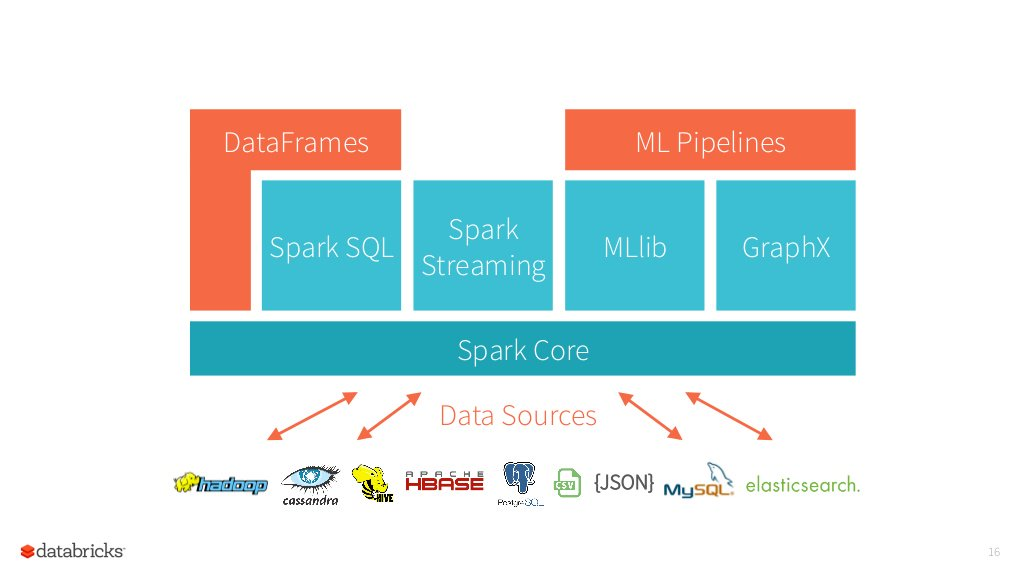
\includegraphics[width=1\textwidth]{images/spark_engine.jpg}
    	\caption{Komponenty frameworku Spark\cite{spark-components}}
    	\label{fig:spark_components}
	\end{figure}
	
\subsubsection{Spark core}
\label{spark-core}
	Tou hlavní komponentou je Spark Core, který zajišťuje všechny základní funkcionality Sparku, jako jsou například plánování úloh a základní vstupní a výstupní operace. Ostatní komponenty nad ním staví. Základním pojmem je zde tzv. Resilient Distributed Dataset, neboli RDD. RDD je zjednodušeně řeřeno téměř libovolná kolekce dat, nad kterou je možné provádět paralelní výpočty. Je navíc zajištěna jejich konzistence - při výpadku některého ze strojů mohou být ztracená data obnova pomocí informací na těch ostatních. 
	
	Kdykoli je na konkrétním RDD vykonána některá z operací umožňujících paralelní zpracování, tzv. transformace (například map, filter nebo reduce), driver neboli počítač řídící ostatní počítače naplánuje její zpracování na všech počítačích v clusteru. Ty poté vytvoří nová RDD s výsledky. Operace na RDD jsou ale "lazy", což znemaná, že se neprovádějí dokud na RDD neaplikujeme nějakou akci. Akce je opakem transformace a jejím výsledkem není vytvoření nového RDD. Příkladem akce je vypsání obsahu RDD na standartní výstup. 

\subsubsection{Spark SQL}
	Další důležitou komponentou je Spark SQL, dříve nazývaný jako Apache Shark. Ten umožňuje práci s především strukturovanými daty. Zavádí také novou strukturu zvanou Data Frame (DF). Stejně jako RDD, je i Data Frame distribuovaný po clusteru. Jeho struktura je ale narozdíl od RDD pevně daná - konceptuelně odpovídá klasické tabulce v relační databázi. Vnitřně v něm dochází k optimalizacím urychlujícím operaci s ním. 
	
	Hlavní předností Spark SQL je možnost používat klasické SQL nebo HiveQL\footnote{An example footnote.} dotazy, jejichž výsledky jsou uloženy právě jako Data Frame. Například komunikace s klasickou relační databází je možná pomocí JDBC/ODBC\footnote{An example footnote.}. 


\subsubsection{Spark Streaming}
	Jak již bylo řečeno, Spark neumožňuje streamové zpracování v pravém slova smyslu, ale pracuje na principu tzv. micro-batchového zpracování. To způsobuje mírné zpoždění výsledků, ty ale nepotřebujeme znát vždy opravdu ihned. Velikou výhodou je fakt, že programy určené pro streamové zpracování se ve Sparku téměř neliší od těch určených k jednorázovému spuštění. 

	\begin{figure}[ht]
    	\centering
    	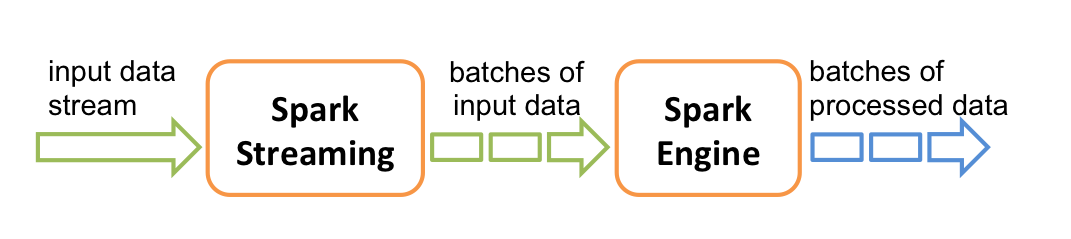
\includegraphics[width=1\textwidth]{images/spark-streaming-flow.png}
    	\caption{Princip fungování Spark Streaming\cite{streaming-guide}}
    	\label{fig:spark_streaming_flow}
	\end{figure}
	
	Jak ukazuje obrázek \ref{fig:spark_streaming_arch}, jako zdroj dat pro Spark Streaming může posloužit například Kafka, Flume, HDFS, Amazon S3 nebo Kinesis. Přímo lze také využívat data z Twitteru bez nutnosti používání dalších knihoven. Právě Twitter poslouží jako zdroj dat pro systém na který se zaměřuje tato práce.  

	\begin{figure}[ht]
    	\centering
    	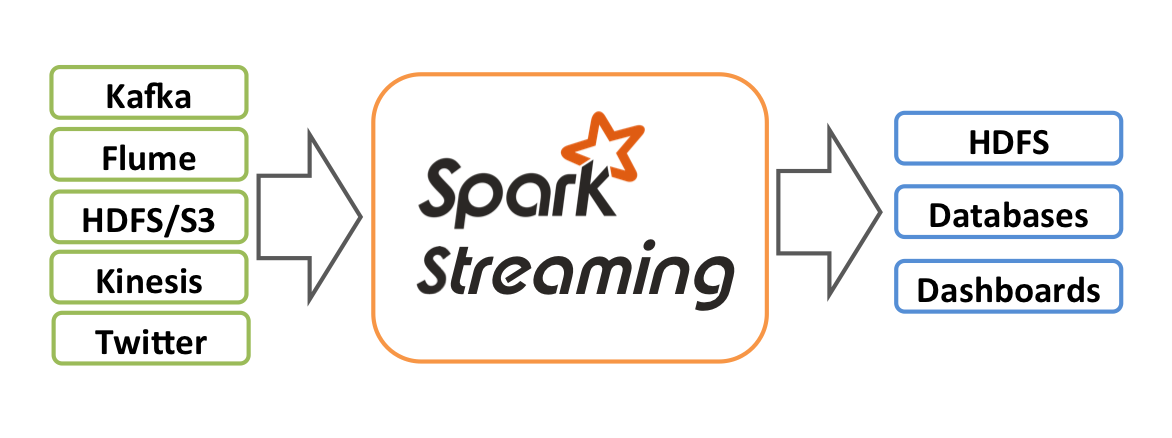
\includegraphics[width=1\textwidth]{images/spark-streaming-arch.png}
    	\caption{Možné zdroje dat a úložiště výsledků pro Spark Streaming\cite{streaming-guide}}
    	\label{fig:spark_streaming_arch}
	\end{figure}
	
	I Spark Streaming zavádí novou strukturu. Nazývá se Discretized Stream neboli DStream. Jde o nekonečnou posloupnost nových dat reprezentovaných jednotlivými RDD. Při psaní konkrétních programů pak stačí nastavit délku intervalu, ve kterém se má opakovaně spouštět daná úloha. DStream pak v každém intervalu dané délky vrátí právě jedno RDD, které je již možné klasicky zpracovat. 
	

\subsubsection{MLlib}
	MLlib je framework určený pro strojové učení. Právě díky vlastnostem Sparku (především díky využívání operační paměti) poskytuje výrazně lepší výsledky než klasické technologie pro machine learning. Výhodou tohoto frameworku je to, že v něm jsou již naimplementovány nejpoužívanější algoritmy. Není tak nutná jejich reimplementace uživatelem. 

	
\subsubsection{Graphx}
	GraphX je ve Sparku relativně novým modulem, který je určený obecně pro práci s grafy a paralelními grafovými výpočty. Grafové výpočty získávají stále více pozornosti, jednoduchým příkladem je algoritmus PageRank, který stál u zrodu moderního vyhledávání v Google\cite{google-pagerank}. 
	


%\section{Způsoby zpracování velkých objemů dat}
%	Batchové/streamové, proc se v mem pripade hodi streamove




\chapter{Analýza}
V této kapitole se nejdříve v sekci \ref{text-mining} věnuji dostupným metodám pro analýzu textu, především pak metodě zvané sentimentální analýza. V sekci \ref{pozadavky} jsou podrobně rozebrány požadavky na implementovaný systém, poslední sekce \ref{twitter} se pak zabývá sociální sítí Twitter a jí poskytovaným rozhraním, které bude v rámci této práce využito. 

\section{Metody pro analýzu textu}
\label{text-mining}
	Získáváním informací z běžného textu se zabývá obor zvaný Text Mining. Jde o obor na pomezí strojového učení a klasického data miningu a umožňuje získávání strukturovaných dat z běžného textu, tedy dat nestrukturovaných. K tomu jsou obvykle použity techniky právě ze zmiňovaných disciplín. Několik základních metod pro dolování dat z textu popisuji v následujících sekcích. 
	
	Protože příspěvky ze sociální sítě Twitter, jejichž analýze se tato práce věnuje, jsou relativně krátké a obsahově specifické, v rámci této práce bude použita pouze metoda zvaná Analýza sentimentu. Té se věnuji nejprve obecně v sekci \ref{sentiment-analysis}. Její použití v kontextu této práce pak podrobněji popisuji v kapitole \ref{analysis-implementation}. 
	
\subsection{Text Categorization}
	Text Categorization, někdy také Text Classification je metodou umožňující rozdělení analyzovaných dokumentů do předem daných skupin, jako například sport, politika a věda. Kategorizace je založena na četnosti jednotlivých slov v analyzovaném textu - pokud například text často obsahuje slova spadající do kategorie sport, bude i celý text do této kategorie zařazen. Rozdělení slov do jednotlivých kategorií je dosaženo buďto manuálně nebo právě pomocí technik strojového učení. Jeden dokument může být obvykle zařezen do více kategorií. 

\subsection{Text Clustering}
	Text Clustering neboli shlukování textů je metoda umožňující seskupování podobných textů. Místo do předem daných kategorií jsou tyto dokumenty přiřazovány na základě jejich podobnosti do dynamicky vytvářených skupin. I zde je rozdělení dosaženo pomocí četnosti jednotlivých použítých slov. Každý dokument je obvykle přiřazen do jediné kategorie. 

\subsection{Document Summarization}
	Vytvářením krátkých shrnujících textů se zabývá metoda zvaná Document Summarization. Jednodušší varianta této metody funguje na principu výběru klíčových vět dokumentu a jejich správného seřazení. Ta složitější pak spočívá v opravdu podrobném rozboru dokumentu, především pak v jeho syntaktické analýze. Ná základě té pak dochází k vytvoření kompletně nového textu shrnujícího text původní. Praktické provedení takové analýzy a následné vytvoření shrnutí je nicméně velice složité a nejsme tak prozatím obvykle schopni dosáhnout tak dobrých výsledků jako pomocí prvně zmíněné varianty\cite{aaaa}. 


\subsection{Sentiment Analysis}
\label{sentiment-analysis}
	Sentiment analysis, v češtině analýza sentimentu, je metodou pro určování celkové nálady či pozitivity daného textu. Výsledkem této analýzy tedy nejsou žádné faktické informace, ale hodnota určující subjektivní názor autora textu na dané téma. 
	
	Jednodušší verze algoritmů pro analýzu sentimentu fungují na podobném principu jako předchozí metody. Text je rozdělen na jednotlivá slova, z nichž každému je přiděleno negativní, neutrální nebo pozitivní hodnocení. Tato hodnocení jsou posléze zprůměrována. Tímto způsobem však dochází ke ztrátě podstatných informací - dochází k zanedbání pořadí slov a především nejsou zohledňovány například negace, které mohou změnit celý význam věty. Příkladem může být následující věta:

\vspace{\baselineskip}
\textit{This movie was actually neither that funny, nor super witty.}	
\vspace{\baselineskip}

	V rámci této práce bude použita knihovna Stanford NLP\cite{sssss}, která mimo jiné obsahuje právě funkce pro analýzu sentimentu. Ty jsou již výrazně propracovanější a výše zmiňovanou větu ohodnotí jako negativní. Podrobněji se použité knihovně věnuji v sekci \ref{stanford-nlp}.


\section{Požadavky na systém}
\label{pozadavky}
	Jak podrobněji popisuji v kapitole \ref{navrh}, výsledný systém jehož vytvoření je cílem této práce se bude skládat ze tří klíčových částí - systému pro analýzu textu, databáze a webserveru zpřístupňujícího data pomocí RESTového API. Pojmu REST API se podrobněji věnuji v sekci \ref{rest}. 
	
	 První zmiňovaná část, systém pro analýzu textu, bude využívat framework Apache Spark. Jako zdroj dat bude použita sociální síť Twitter poskytující vzorek přispěvků z ní, tzv. tweetů, pomocí veřejného API. Tomu se podrobněji věnuji v kapitole \ref{twitter-api}. Z těchto příspěvků budou vyfiltrovány ty, které reprezentují přání jejich autorů. Kromě měření běžných statistik bude systém provádět analýzu sentimentu těchto přání. Tato analýza bude probíhat v reálném čase, respektive se zpožděním v řádu maximálně několika desítek sekund.  Výsledky analýzy z této části budou persistovány ve vhodné relační databázi. Na ní bude napojen webový server zpřístupňující data pomocí RESTful API. 

\subsection{Funkční požadavky}
\subsubsection{Systém pro analýzu textu}
Samotný systém pro analýzu textu musí splňovat následující požadavky:
\begin{itemize}
\item Získání a ukládání veškerých dat, jejichž zpřístupnění pomocí RESTového API je požadováno a jež nejsou získávána jiným způsobem
\end{itemize}
\subsubsection{Databáze}
 Databáze bude poskytovat následující funkcionality:
\begin{itemize}
\item Agregace statistických dat dle času - u dat u kterých je to možné bude docházet k jejich seskupovaní po větších intervalech. Tím dojde ke snížení náročnosti dotazů na tato data. 
\item Promazávání starých a již zagregovaných dat
\end{itemize}
\subsubsection{RESTful API}
RESTful API bude poskytovat následující data:

\begin{itemize}
\item Jednotlivá přání a základní informace o nich, včetně jejich sentimentu a informací o jejich autorovi
\item Seznam uživatelů zmíněných v konkrétním přání
\item Seznam hastagů použitých v konkrétním přání
\item Informace o uživatelích, kteří jsou autory některého přání nebo byli v některém zmíněni
\item Seznam přání publikovaných daným uživatelem
\item Seznam přání v nichž byl daný uživatel zmíněn
\item Seznam přání obsahujících daný hashtag
\item Statistiky nejpouívanějších hashtagů
\item Statistiky nejvíce zmiňovaných uživatelů
\item Statistiky o počtech již analyzovaných tweetů, anglických tweetů a z nich vyfiltrovaných přání v daném časovém intervalu
\item Statistika o průměrném sentimentu v daném intervalu
\end{itemize}

\noindent Pro data pro která je to vhodné bude API umožňovat:
\begin{itemize}
\item Omezení počtu vrácených výsledků
\item Nastavení časového intervalu
\item Poskytnutí pouze některých hodnot, například pouze statistik počtu anglických tweetů namísto veškerých statistických údajů
\end{itemize}

\subsection{Nefunkční požadavky}
\subsubsection{Kvalitativní}
\begin{itemize}
\item \textbf{Rychlost} - analýza textu bude probíhat v reálném čase, respektivě se zpožděním v řádu maximálně několika desítek sekund
\item \textbf{Škálovatelnost} - systém pro analýzu textu bude při nasazení na dostatečně výkoném počítačovém clusteru připraven pro zpracování tisíců příspěvků za sekundu
\end{itemize}
\subsubsection{Omezující}
\begin{itemize}
\item \textbf{Framework pro analýzu} - k analýze příspěvků z Twitteru bude použit framework Apeche Spark a jeho komponenta Spark Streaming
\item \textbf{Zpřístupnění dat} - data budou zpřístupněna pomocí RESTful API. To bude odpovídat běžným praktikám používaným právě při návrhu RESTových rozhraní
\end{itemize}

\section{Sociální síť Twitter}
\label{twitter}
	
	Twitter je v současnosti jednou z nejpoužívanějších sociálních sítí poskytující svým uživatelům mikroblogovací funkcionality. Umožňuje zveřejňovat 140 znaků dlouhé zprávy (tzv. tweety) a číst zprávy publikované ostatními. Účet na něm má odhadem 1,3 milardy uživatelů, denně se jich pak na Twitter přihlásí asi 100 milionů\cite{twitter-stats}. Tito uživatelé pak každý den zveřejní 500 milionů tweetů, což odpovídá približně 6000 tweetů každou sekundu\cite{twitter-stats-2}. 

\subsection{Vysvětlení pojmů}
Pro bližší pochopení fungování sociální sítě Twitter a analýzy příspěvků z ní pro účely této práce je potřeba vysvětlit několik základních termínů:

\subsubsection{Tweet}

Tweet je tím nejdůležitejším pojmem na Twitteru. Jak již bylo řečeno, jedná se o zprávu o maximální délce 140 znaků. Důvody pro toto omezení jsou v dnešní době víceméně historické - Twitter byl totiž už od svých počátků zamýšlen pro použití na mobilních telefonech. Protože klasické textové zprávy posílané právě pomocí mobilních telefonů jsou omezeny na 160 znaků, bylo toto omezení při vzniku Twitteru bráno v potaz. Samotný 140 znaků dlouhý tweet by zabral většinu délky SMS zprávy, zbylých 20 znaků bylo vyhrazeno pro jméno autora zprávy\cite{twitter-140}. Nicméně i dnes má toto omezení smysl - nutí uživatele zprávy zkracovat a zmiňovat to nejdůležitější. 

Všechny tweety zveřejněné uživatelem jsou standartně viditelné pro všechny. Uživatel však má možnost nastavit si vyšší úroveň soukromí. Přímo na hlavní stránce se uživateli zobrazují příspěvky těch uživatelů, jejichž je tzv. follower. 

\subsection{Follower}

	Followerem neboli "sledujícím" jiného uživatele se člověk stane jednoduše kliknutím na tlačítko Follow na profilu vybraného uživatele. To způsobí právě zobrazování zpráv sledovaného uživatele na hlavní stránce Twitteru. Sledovaný uživatel si může zobrazit seznam uživatelů kteří ho sledují. 


\subsubsection{Retweet}

	Často používanou funkcionalitou Twitteru je možnost přeposlat zprávy někoho jiného neboli vytvořit tzv. retweet. Taková zpráva pak začíná písmeny RT označujícími právě retweet, za nimi pak následuje jméno původního autora zprávy. 


\subsubsection{Hashtag}

	Hashtag je řetězec začínající znakem "\#". Hashtagy vkládají samotní uživatelé do jimi publikovaných tweetů. Na základě použitého hashtagu je pak možno vyhledat i ostatní zprávy, které ho obsahují. Příkladem může být hashtag \#rio2016 používaný pro tweety týkající se nadcházejících Olympijských her v Brazilském Rio de Janeiru. Dostupné hashtagy však nejsou nijak omezeny, použit může být libovolný řetězec. 


\subsubsection{Mention}

	Stejně jako může tweet obsahovat hashtag, může v něm být zmíněný jiný uživatel Twitteru. Toto zmínění je v originále označováno jako tzv. Mention. Pro zmínění jiného uživatele je použit znak zavináče následovaný uživatelským jménem. 


\subsection{Twitter Streaming API}
\label{twitter-api}
	Twitter poskytuje 2 rozhraní pro přistup k jeho datům. Jde o klasické REST API s mnoha různými endpointy\footnote{Endpoint neboli koncový bod je ......} a dále o několik streamových endpointů. Tato práce využívá stremové API, konkretně stream poskytující vzorek veřejně publikovaných tweetů\cite{twitter-api}. Počet tweetů které toto API poskytuje není přesně daný, nicméně experimentálně bylo zjištěno, že jde o přibližně 60 až 80 příspěvků za sekundu. To odpovídá asi 1\% publikovaných tweetů. 
	
	Získat lze samozřejmě i přístup ke všem veřejně publikovaným příspěvkům. Nejde však již o volně dostupná API a přístup k nim je placený. Tuto službu nabízí portál Gnip.com\cite{gnip}. Pro tuto práci je z pocohpitelných důvodů použito pouze veřejně dostupné API. 
	
	Pro různé případy užití se hodí využít jiné rozhraní. Klasický případ vužití RESTového API ukazuje obrázek \ref{fig:twitter_rest} - uživatel navštíví webovou stránkou a chce zobrazit například údaje o konkrétním uživateli. Server tento požadavek přijme a sám odešle požadavek na API poskytované Twitterem. Ten mu odpoví, server data zpracuje a vrátí je původnímu uživateli. 

\begin{figure}[ht]
   	\centering
   	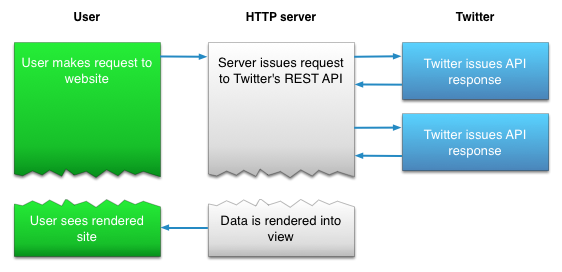
\includegraphics[width=1\textwidth]{images/twitter-rest.png}
   	\caption{Schéma fungování klasického Twitter REST API\cite{twitter-rest-stream}}
   	\label{fig:twitter_rest}
\end{figure}

	V některých případech je ale vhodnější využít právě streaming API. Pokud nepotřebujeme okamžitě reagovat na jednotlivé požadavky uživatelů ale naopak chceme data zpracovávat kontinuelně, je streaming API jasnou volbou. Mimo jiné díky němu dosáhneme nižšího zatížení serveru, protože není nutné neustálne navazovat nová spojení. Tento princip je popsán na obrázku \ref{fig:twitter_streaming}. 

\begin{figure}[ht]
   	\centering
   	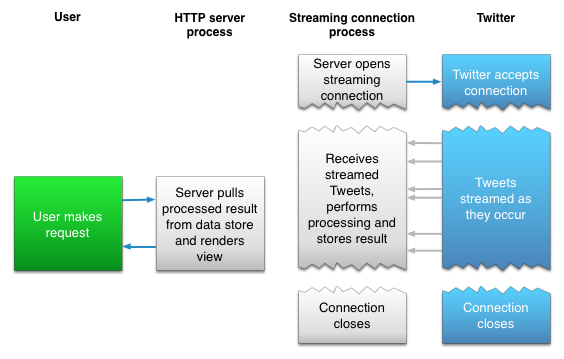
\includegraphics[width=1\textwidth]{images/twitter-streaming.png}
   	\caption{Schéma fungování Twitter Streaming API\cite{twitter-rest-stream}}
   	\label{fig:twitter_streaming}
\end{figure}


\subsubsection{Twitter4j}
	Popisovat konkrétní parametry použitého streaming API nemá v kontextu této práce smysl. Spark streaming má totiž v sobě Twitter Streaming API zaintegrované jako jeden z možných zdrojů dat a veškerou práci s API tak řeší za uživatele. Je pouze třeba nastavit přístupové údaje k API, které je možné získat vytvořením vývojářského Twitter účtu. 
	
	Spark navíc využívá java knihovnu Twitter4j\cite{twitter4j}, která usnadňuje práci s Twitter API. Díky tomu jsou jednotlivá RDD tvořena již přímo objekty reprezentující jednotlivé tweety. Pomocí metod těchto objektů je pak možné o každém tweetu snadno získat všechny dostupné informace, včetně například údajů o autorovi tweetu. 


\chapter{Návrh}
\label{navrh}
V této kapitole se věnuji návrhu jednotlivých komponent implementovaného systému. Jak již bylo nastíněno v definici požadavků, bude se tento systém skládat z několika hlavních částí: 
\begin{itemize}
\item \textbf{Systém pro analýzu tweetů} využívající framework Spark bude sloužit k analýze příspěvků ze sociální sítě Twitter. Po vyfiltrování tweetů reprezentujích přání jejich autorů provede analýzu sentimentu těchto tweetů. Výsledky analýzy společně s obecnými údaji o zpracovávaných textech budou uloženy do databáze. 
\item \textbf{Databáze} bude uchovávat veškeré potřebné údaje o analyzovaných příspěvcích. Krom toho bude v databázi docházet k agregaci dat pro dosažení snížené zátaže. 
\item \textbf{Webserver poskytující REST API} bude zpřístupňovat veškeré údaje, jejichž dostupnost je vyžadována ve funkčních požadavcích. 
\item \textbf{Webová aplikace} sice není součástí zadání této práce, bude nicméně z důvodů prezentace výsledků a testování API také implementována. 
\end{itemize}

\noindent Jednotlivé části podrobněji popisuji v následujících sekcích. 

\section{Analýza tweetů}
	Program pro analýzů tweetů bude klíčovou částí celkového systému. Bude v něm totiž docházet ke zpracování veškerých dat. Hlavními cíli této komponenty jsou:
	
\begin{itemize}
\item \textbf{Vyfiltrování anglických přání.} Příspěvky publikované na Twitteru jsou napsány v různých jazycích, tento systém bude však provádět analýzu pouze těch anglických. Je proto nejprve nutné anglické příspěvky vyfiltrovat. Samotné vyfiltrování příspěvků reprezentujících přání jejich autorů pak bude provedeno jednoduše nalezením tweetů obsahujících slova \textit{wish}, \textit{hope} nebo \textit{pray}. 
\item \textbf{Ukládání přání a souvisejících údajů.} Veškerá vyfiltrovaná přání a dále údaje o jeho autorovi, zmíněných uživatelých a obsažených hashtazích budou ukládány do databáze. 
\item \textbf{Provedení analýzy sentimentu jednotlivých přání.} U veškerých vyfiltrováních přání bude provede analýza sentimentu, jejíž výsledky budou taktéž uloženy do databáze. 
\item \textbf{Ukládání obecných statistik.} Během zpracování budou ukládány také obecné statistiky o počtech zpracovaných příspěvků a průměrném sentimentu v daném časovém intervalu. 
\end{itemize}

\section{Struktura databáze}
Databáze uchovávající výsledky analýzy dat musí pojmout všechna data, jejichž zpřístupnění je dle funkčních požadavků vyžadováno. Konkrétní strukturu databáze ukazuje obrázek \ref{fig:db-structure}. 

\begin{figure}[ht]
   	\centering
   	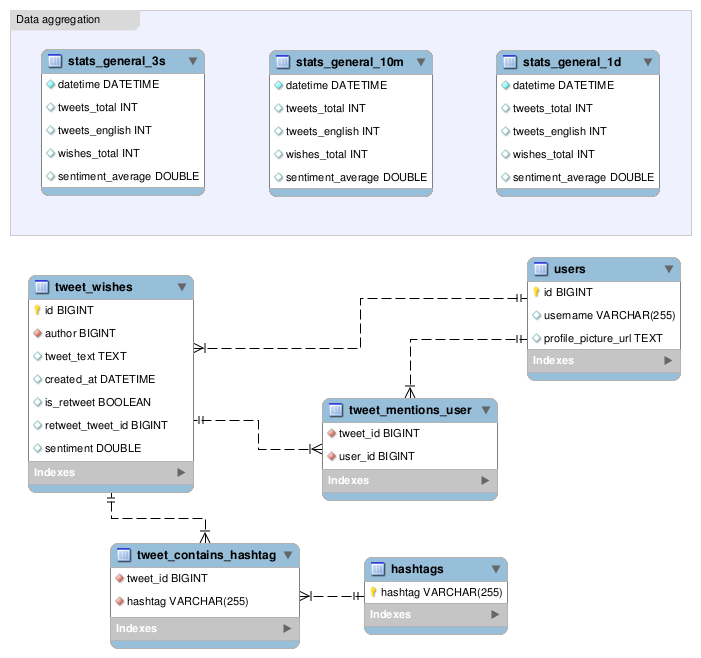
\includegraphics[width=1\textwidth]{../db_model.png}
   	\caption{Návrh schámatu databáze}
   	\label{fig:db-structure}
\end{figure}

V horní části obrázku jsou umístěny tabulky uchovávající obecné statistiky o zpracovaných datech. Z nich pouze do první tabulky \textit{stats\_general\_3s} bude přímo vkládat data systém pro analýzu textu. Zbylé dvě tabulky budou obsahovat agregovaná data, jak vysvětluji v sekci \ref{agregace-dat}. 

Krom obecných statistik budou ukládána veškerá analyzovaná přání včetně výsledku jejich sentimentální analýzy. V tabulce \textit{users} pak budou uloženy základní údaje o všech uživatelích, kteří jsou autory některého z analyzovaných přání nebo jsou v něm zmíněni. Vztah vyjadřující zmínění uživatele v tweetu bude vyjádřen tabulkou \textit{tweet\_mentions\_user}. 

Stejně tak jsou tabulce \textit{hashtags} uloženy všechny hashtagy použité v některém z přání. Použití hashtagu v přání vyjadřuje tabulka \textit{tweet\_contains\_hashtag}.

\section{Návrh API}
\label{rest}
\subsection{REST architektura}
	Jedním z požadavků pro API poskytující výsledky analýzy dat je využití REST neboli Representational State Transfer architektury. Tato architektura rozhraní byla představena v roce 2000 Royem Fieldingem, spoluautorem protokolu HTTP\cite{jjjlkll}. Proto není překvapením že REST pro přenos dat využívá právě tento protokol. Jedná se o bezestavovou architekturu, která poskytuje jednoduchý a především jednotný přístup ke zdrojům. Za zdroj pak považujeme samotná data či stavy aplikace. 
	
	Každý zdroj má svoji vlastní URI\footnote{URI}, REST definuje čtyři základní metody pro přístup k nim. Tyto základní metody protoklu HTTP jsou označovány jako CRUD - umožňují totiž vytvoření dat (Create), jejich získání (Retrieve), aktualizování (Update) a smazání (Delete):
\begin{itemize}

\item\textbf{GET}

Get je tou nejzákladnější metodou, která slouží k získání zdroje. Při používání webového prohlížeče se s ním setkáváme neustále - jedná se totiž o metodu sloužící jako klasický požadavek na webovou stránku. Případné parametry jsou přidány přimo do URI. Pro získání informají o uživateli Jan můžeme použít následující požadavek: 
\begin{lstlisting}[frame=single]
GET /api/user/jan
Host: www.my-web.com
\end{lstlisting}

\item\textbf{POST}

Post je metoda sloužící pro vytváření dat nových, která se používá například u klasických webových formulářů. Parametry s údaji pro nová data nejsou součástí URI ale přímo HTTP dotazu. 

\item\textbf{DELETE}

Metoda Delete slouží ke smazání konkrétního zdroje definovaného pomocí URI. HTTP požadavek pro smazání uživatele Jan by se nelišil od výše uvedeného příkladu požadavku GET, pouze by bylo nutné použít metodu DELETE. 

\item\textbf{PUT}

Put je metodou sloužící k aktualizaci zdroje. Jde jistým způsobem o kombinaci GET a POST - používá přímo URI již existujícího zdroje jako GET, ale v těle HTTP požadavku odesílá nová data sloužící k aktualizaci tohoto zdroje. 

\end{itemize}

	
\subsection{JSON}	
	Jedním z nejčastěji používaných formátů pro přenos dat v kombinaci s RESTovým API je JSON, neboli JavaScript Object Notation. Použit bude i v rámci této práce. Skládá se z dvojic klíčů a hodnot a jeho hlavními výhodami jsou jednoduchá struktura, přehlednost a čitelnost. 
	
	Většina programovacích jazyků navíc obsahuje knhovny a funkce, které umožňují jednoduché zpracování tohoto formátu. Například v jazyce Python formát JSON v podstatě odpovídá klasickému slovníku. Následující ukázka zobrazuje zápis objektu obsahujícího pole se dvěma uživateli:
\begin{lstlisting}[language=json,firstnumber=1]
{
	"users": [{
		"name": "Jan Novak",
		"age": 24,
		"address": {
			"city": "Praha 7",
			"street": "Dlouha",
			"street_number": "451"
		}
	}, {
		"name": "Karel Spacek",
		"age": 46,
		"address": {
			"city": "Praha 4",
			"street": "Siroka",
			"street_number": "841"
		}
	}]
}
\end{lstlisting}
	
\subsection{API enpointy}
	Kromě použití architektury REST je také nutné splnit všechny funkční požadavky definované v sekci \ref{pozadavky}. Jelikož API data pouze zpřístupňuje ale nikterak je neupravuje, veškeré API endpointy budou využívat pouze výše popsanou metodu GET. Podrobný popis implementovaných API endpointů je možné najít v příloze \ref{appendix-api}. Zjednodušený popis je pak dostupný přímo zde: 
	

\begin{table}[h]
\begin{tabular}{llllr}
\rowcolor[HTML]{EFEFEF}
\large \textbf{/wish/}        &         &                 &        & \multicolumn{1}{l}{}                \\
\rowcolor[HTML]{EFEFEF}
\textbf{GET}          &         &                 &        & Seznam přání                        \\
\multicolumn{5}{l}{\parbox[t]{12.8cm}{Bez použití následujích parametrů vrátí všechna přání za posledních 10 minut. Při použití \textit{count} jsou ignorovány parametry  \textit{from} a \textit{to}.}  } \\
\textbf{from}         &         & timestamp       &        & od včetně                           \\
\textbf{to}           &         & timestamp       &        & do vyjímaje                         \\
\textbf{count}        &         & integer         &        & omezení počtu vrácených přání      \\
\end{tabular}
\end{table}



\begin{table}[h]
\begin{tabular}{llllr}
\rowcolor[HTML]{EFEFEF}
\large \textbf{/wish/\{wish\_id\}}        &         &                 &        & \multicolumn{1}{l}{}                \\
\rowcolor[HTML]{EFEFEF}
\textbf{GET}          &         &                 &        & Konkrétní přání                        \\
\multicolumn{5}{l}{\parbox[t]{12.8cm}{Vrací stejné údaje jako \textit{/wish/}, ale pouze pro konkrétní přání s daným \textit{wish\_id}.}  } \\  
\end{tabular}
\end{table}
 

\begin{table}[h]
\begin{tabular}{llllr}
\rowcolor[HTML]{EFEFEF}
\large \textbf{/wish/\{wish\_id\}/mentions}        &         &                 &        & \multicolumn{1}{l}{}                \\
\rowcolor[HTML]{EFEFEF}
\textbf{GET}          &         &                 &        & Uživatelé zmíněný v přání                        \\
\multicolumn{5}{l}{\parbox[t]{12.8cm}{Vrací seznam uživatelů zmíněných v přání s daným \textit{wish\_id}.}  } \\    
\end{tabular}
\end{table}


\begin{table}[h]
\begin{tabular}{llllr}
\rowcolor[HTML]{EFEFEF}
\large \textbf{/wish/\{wish\_id\}/hashtags}        &         &                 &        & \multicolumn{1}{l}{}                \\
\rowcolor[HTML]{EFEFEF}
\textbf{GET}          &         &                 &        & Hashtagy použité v přání                        \\
\multicolumn{5}{l}{\parbox[t]{12.8cm}{Vrací seznam hashtagů použitch v přání s daným \textit{wish\_id}.}  } \\    
\end{tabular}
\end{table}

\begin{table}[h]
\begin{tabular}{llllr}
\rowcolor[HTML]{EFEFEF}
\large \textbf{/user/}        &         &                 &        & \multicolumn{1}{l}{}                \\
\rowcolor[HTML]{EFEFEF}
\textbf{GET}          &         &                 &        & Seznam uživatelů                        \\
\multicolumn{5}{l}{\parbox[t]{12.8cm}{Vrací seznam všech uživatelů, tedy autorů přání nebo uživatelů zmíněných v některém z nich. }  } \\   
\end{tabular}
\end{table}


\begin{table}[h]
\begin{tabular}{llllr}
\rowcolor[HTML]{EFEFEF}
\large \textbf{/user/\{user\_id\}}        &         &                 &        & \multicolumn{1}{l}{}                \\
\rowcolor[HTML]{EFEFEF}
\textbf{GET}          &         &                 &        & Konkrétní uživatel                        \\
\multicolumn{5}{l}{\parbox[t]{12.8cm}{Vrací údaje o konkrétním uživateli s daným \textit{user\_id}. }  } \\  
\end{tabular}
\end{table}


\begin{table}[h]
\begin{tabular}{llllr}
\rowcolor[HTML]{EFEFEF}
\large \textbf{/user/\{user\_id\}/wishes}        &         &                 &        & \multicolumn{1}{l}{}                \\
\rowcolor[HTML]{EFEFEF}
\textbf{GET}          &         &                 &        & Přání daného uživatele                        \\
\multicolumn{5}{l}{\parbox[t]{12.8cm}{Vrací seznam přání uživatele s daným \textit{user\_id}. }  } \\  
\end{tabular}
\end{table}

\begin{table}[h]
\begin{tabular}{llllr}
\rowcolor[HTML]{EFEFEF}
\large \textbf{/user/\{user\_id\}/mentioned\_in}        &         &                 &        & \multicolumn{1}{l}{}                \\
\rowcolor[HTML]{EFEFEF}
\textbf{GET}          &         &                 &        & Zmínění daného uživatele                        \\
\multicolumn{5}{l}{\parbox[t]{12.8cm}{Vrací seznam přání, ve kterých byl uživatel s daným \textit{user\_id} zmíněn. }  } \\  
\end{tabular}
\end{table}


\begin{table}[h]
\begin{tabular}{llllr}
\rowcolor[HTML]{EFEFEF}
\large \textbf{/hashtag/\{hashtag\}/wishes}        &         &                 &        & \multicolumn{1}{l}{}                \\
\rowcolor[HTML]{EFEFEF}
\textbf{GET}          &         &                 &        & Přání obsahující daný hashtag                       \\
\multicolumn{5}{l}{\parbox[t]{12.8cm}{Vrací seznam přání, ve kterých byl použit daný \textit{hashtag}. }  } \\  
\end{tabular}
\end{table}

\begin{table}[h]
\begin{tabular}{llllr}
\rowcolor[HTML]{EFEFEF}
\large \textbf{/stats/mentions}        &         &                 &        & \multicolumn{1}{l}{}                \\
\rowcolor[HTML]{EFEFEF}
\textbf{GET}          &         &                 &        & Seznam zmiňovaných uživatelů                        \\
\multicolumn{5}{l}{\parbox[t]{12.8cm}{Bez použití následujích parametrů vrátí seznam všech zmíněných uživatelů v posledních 10 minutách společně s počtem jejich zmínění. \\ Výsledky jsou řazeny sestupně dle počtu zmínění v daném intervalu. }  } \\
\textbf{from}         &         & timestamp       &        & od včetně                           \\
\textbf{to}           &         & timestamp       &        & do vyjímaje                         \\
\textbf{count}        &         & integer         &        & omezení počtu vrácených uživatelů     \\ 
\end{tabular}
\end{table}


\begin{table}[h]
\begin{tabular}{llllr}
\rowcolor[HTML]{EFEFEF}
\large \textbf{/stats/hashtags}        &         &                 &        & \multicolumn{1}{l}{}                \\
\rowcolor[HTML]{EFEFEF}
\textbf{GET}          &         &                 &        & Seznam používaných hashtagů                        \\
\multicolumn{5}{l}{\parbox[t]{12.8cm}{Bez použití následujích parametrů vrátí seznam všech hashtagů použitých v posledních 10 minutách společně s počtem jejich použití. \\ Výsledky jsou řazeny sestupně dle počtu použití v daném intervalu. }  } \\
\textbf{from}         &         & timestamp       &        & od včetně                           \\
\textbf{to}           &         & timestamp       &        & do vyjímaje                         \\
\textbf{count}        &         & integer         &        & omezení počtu vrácených hashtagů     \\
\end{tabular}
\end{table}


\begin{table}[h]
\begin{tabular}{llllr}
\rowcolor[HTML]{EFEFEF}
\large \textbf{/stats/general}        &         &                 &        & \multicolumn{1}{l}{}                \\
\rowcolor[HTML]{EFEFEF}
\textbf{GET}          &         &                 &        & Obecné statistiky                        \\
\multicolumn{5}{l}{\parbox[t]{12.8cm}{Bez použití následujích parametrů vrátí obecné statistiky za posledních 10 minut.  }  } \\
\textbf{from}         &         & timestamp       &        & od včetně                           \\
\textbf{to}           &         & timestamp       &        & do vyjímaje                         \\
\textbf{density}        &         & "3s"/"10m"/"1d"         &        & hustota statistických dat   \\
\end{tabular}
\end{table}


\chapter{Implementace}
\label{implementace}
V následujících sekcích jsou podrobněji popsány způsoby implementace jednotlivých částí systému. Způsob jeho nasazení je znázorněn na obrázku \ref{fig:deployment_diagram}. Z důvodů zmíněných v sekci \ref{analysis-implementation} byl však místo počítačového clusteru použit virtualizovaný systém na lokálním počítači. 

Při vývoji systému i psaní tohoto textu byl používán verzovací systém GIT. Repozitář této práce je možné nalézt na serveru GitHub\cite{ghrtyrtt}. 

\begin{figure}[h!]
   	\centering
   	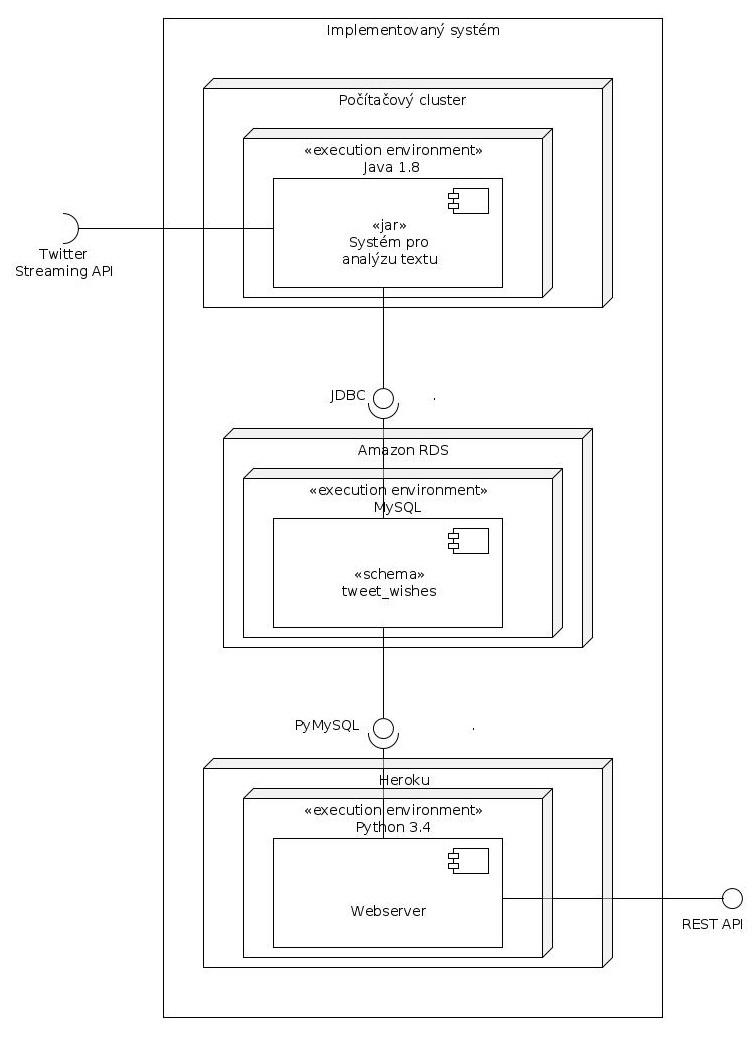
\includegraphics[width=1\textwidth]{images/deployment.jpg}
   	\caption{Diagram nasazení implementovaného systému}
   	\label{fig:deployment_diagram}
\end{figure}

\section{Analýza proudu dat}
\label{analysis-implementation}
\subsection{Výběr technologií}
Framework Spark, který byl použit při implementaci analýzy proudu dat, nabízí API pro několik jazyků - Scala, Java, Python a R. API pro poslední dva zmiňované jazyky však neposkytují veškeré funkcionality Sparku, příkladem může být použití Twitter Streaming API jako zdroje dat. V úvahu pro použití v rámci této práce tedy připadaly jazyky Java a Scala. 

Jak již bylo zmíněno v kapitole \ref{spark-core}, výpočty lze distribuovat pro operace typu transformace, tedy například map, filter a reduce. Protože Scala je funkcionální jazyk obsahující podobné funkce již v základu, je v kontextu distribuovaných výpočtů ideální. I proto je samotný Spark naimplementovaný ve Scale\cite{kkkkjjjhh}. Další výhodou je možnost použití existujících knihoven pro Javu. Především z těchto důvodů byla Scala použita i pro tuto práci. 

\subsubsection{Stanford NLP knihovna}
\label{stanford-nlp}
	Pro analýzu sentimentu byla namísto vlastní jednoduché implementace analýzy sentimentu použita Java knihovna Stanford NLP\cite{fghjkkl}. Jedná se o knihovnu obecně poskytující funckionality pro zpracování a analýzu lidské řeči. Zahrnuje právě analyzátor pro určení sentimentu. 
	
	Použitý model je nejdříve potřeba vytrénovat na vzorových datech. Bez manuálního přetrénování je algoritmus již vytrénován na datasetu složeného z necelých 10 tisíc vět z oblasti filmových hodnocení. Tato trénovací data je možné najít na stránce Stanford Dataset Treebank\cite{ssdassa}. V rámci této práce nebude použitý model přetrénováván přímo pro kontext sociální sítě Twitter, bylo by totiž potřeba manuálně ohodnotit řádově tisíce vět. 
	
	Výsledkem analýzy sentimentu pomocí Stanford NLP je hodnota v intervalu 0 až 4, kde 0 reprezentuje negativní a 4 pozitivní větu. Jednotlivé tweety tedy bylo nutné rozdělit na věty a každou z nich analyzovat zvlášť. Celkový sentiment tweetu byl pak určen na základě hodnocení jednotlivých vět a jejich délce. 

\subsection{Nasazení}
Aby implementovaný systém zvládal analyzovat všechny publikované tweety, bylo by nutné jeho nasazení na počítačovém clusteru. K tomu je systém připravený a krom instalace potřebného software na jednotlivé stroje by nasazení nemělo vyžadovat další úpravy zdrojových kódů. Jak jsem ale popsal v sekci \ref{twitter-api}, ve volně dostupném API Twitter poskytuje pouze asi 1\% publikovaných zpráv. Protože navíc počítačový cluster nemám k dispozici a jeho pronájem by byl velice nákladný, je program spouštěn na lokálním počítači ve virtualizovaném prostředí. 

K dispozici má Spark 8GB RAM a 3 výpočetní jádra. Je ho možné spustit v tzv. lokálním režimu, ve kterém je na každém jádře spuštěn jeden výpočetní uzel. I kvůli omezeným zdrojům bylo v průběhu implementace nutné zvětšit délku intervalu, ve kterém Spark data zpracovává. Většina tohoto času je však overhead a s nárůstem objemu zpracovávaných dat není celková doba jejich analýzy výrazně navýšena. 

\subsection{Popis implementace}

Celkový pohled na implementovaný systém zobrazuje diagram aktivit na obrázku \ref{fig:activity_diagram}. Po úspěšné inicializaci Sparku a přihlášení k Twitter Streaming API začnou probíhat dvě nezávislé větve programu. Samotné střádání dat z Twitteru vždy po dobu 40 vteřin řeší samotný Spark. Po uběhnutí daného intervalu jsou data poskytnuta jako RDD ke zpracování a ihned začíná další střádání dat. 

Druhá větev má za úkol zpracování dat poskytnutých větví první. Ke zpracování další batche dochází kdykoli je dokončeno zpracování té předchozí a zároveň jsou k dispozici nová data. Program se tak může dostávat do zpoždění pokud data zpracovávat nestíhá v daném intervalu. Při zpracování dat z každého intervalu jsou nejprve vyfiltrovány anglické příspěvky reprezentující přání jejich autorů. Poté je vypočítán sentiment těchto přání a data o nich jsou uložena do databáze. 

Několik zajímavých částí této implementace zobrazují následující zdrojové kódy. Před začátkem zpracování dat je krom připojení k Twitteru také potřeba provést základní nastavení Sparku. Nutné je především vytvořit kontexty, jak ukazuje zdrojový kód \ref{fig:spark-context}. Tyto kontexty budou později použity při operacích prováděných při zpracování dat. Vytvořen je také samotný stream. 

\begin{figure}
\begin{lstlisting}[language=json,firstnumber=1][h]
val conf = new SparkConf().setAppName("Twitter Wishes Analysis")

val sc = new SparkContext(conf)
val ssqlc = new SQLContext(sc)
val ssc = new StreamingContext(sc, Seconds(40))

val stream = TwitterUtils.createStream(ssc, None)
\end{lstlisting}
\caption{Vytvoření kontextů a streamu}
\label{fig:spark-context}
\end{figure} 

Z vytvořeného streamu je potřeba vyfiltrovat pouze anglické příspěvky. K tomu je použita metoda \textit{getLang()} dostupná v knihovně Twitter4j. Zdrojový kód \ref{fig:spark-filter} ukazuje také vyfiltrování pouze příspěvků reprezentujících přání jejich autorů. 

\begin{figure}
\begin{lstlisting}[language=json,firstnumber=1][h]
// filter English tweets
var tweetWishesStream = stream.filter( status => ( status.getLang() == "en"))

// filter wishes
tweetWishesStream = tweetWishesStream
	.filter( status => (
		status.getText().contains("wish") ||
		status.getText().contains("hope") ||
		status.getText().contains("pray") ))
\end{lstlisting}
\caption{Vyfiltrování anglických přání}
\label{fig:spark-filter}
\end{figure} 

V další části již nastává samotná analýza vyfiltrovaných přání. Zdrojový kód \ref{fig:spark-stats-db} zobrazuje vytvoření DataFramu obsahujícího obecné statistiky v daném časovém intervalu a jejich uložení do databáze. 

\begin{figure}
\begin{lstlisting}[language=json,firstnumber=1][h]
// write stats to DB
val stats = ssqlc.createDataFrame(Seq((currentDatetime, tweetCount,
	tweetCountEnglish, wishCount, average_sentiment)))
	.toDF("datetime",
		"tweets_total",
		"tweets_english",
		"wishes_total",
		"sentiment_average")
stats.write.mode(SaveMode.Append).jdbc(DBUrl, "stats_general_3s", prop)
\end{lstlisting}
\caption{Ukládání statistik do databáze}
\label{fig:spark-stats-db}
\end{figure} 
	
\begin{figure}[h]
   	\centering
   	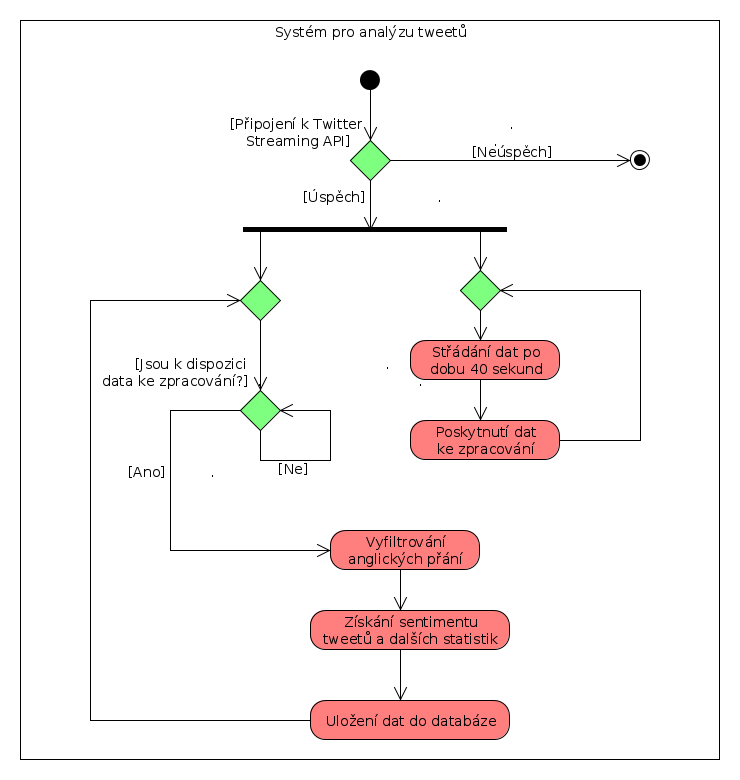
\includegraphics[width=1\textwidth]{images/activity-diagram.png}
   	\caption{Diagram aktivit systému pro analýzu tweetů}
   	\label{fig:activity_diagram}
\end{figure}

\section{Databáze}
\subsection{Výběr technologií}
	Při výběru konkrétní databáze bylo nejdříve nutné rozhodnout, zda použít klasickou relační databázi nebo sáhnout po NoSQL databázi. NoSQL databáze, někdy také označované jako Not Only SQL, zpravidla nejsou relační a nemají pevně dané schéma. Na druhou stranu tyto databáze nabízejí větší možnosti škálování, často jsou distribuované a umožňují pojmout výrazně větší objemy dat než databáze klasické\cite{nosql-dbs}. 
	
	Data jsou v nich obvykle uložena ve formátu podobném JSONu, přičemž narozdíl od relačních databázích často provádíme jejich denormalizaci. To umožňuje rychlejší načtení informací z databáze, aktualizace dat je ale naopak časově náročnější. NoSQL databáze se často využívají právě v projektech pracujících s Big Daty. Jednou z nejrozšířenějších NoSQL databází je Cassandra. 
	
	Z několika důvodů jsem však pro tuto práci zvolil klasickou relační databázi. Po vyfiltrování jednotlivých přání a jejich analýze nebudu pracovat s tak velkými objemy dat, které by relační databáze nebyla schopna pojmout. Tato data navíc mezi sebou mají jasné vztahy, které je možné zanést do schématu databáze a usnadnit si tak práci s nimi. Relační databáze jsou také využívány výrazně delší dobu a jsou vývojově vyspělejší. 
	
	Z volně dostupných databázových řešení jsou nejrozšířenější především MySQL a PostgreSQL. Protože tato práce neklade na databázi žádné specifické požadavky, výběr konkrétní databáze je možné založit pouze na obecných parametrech. Protože PostgreSQL nabízí některé funkcionality které MySQL nebsahuje a protože je obecně považována za databázi na lepší úrovni\cite{aaaaaaaa}, bylo PostgreSQL první volbou i pro tuto práci. Po několika neúspěšných pokusech propojit právě PostgreSQL s frameworkem Apache Spark však bylo nutné použít MySQL. 
	
\subsection{Nasazení databáze}
	Po výběru konkrétních databázových technologií byl potřeba zvolit vhodný způsob nasazení. Z důvodů popsaných v následující sekci nebyl k nasazení použit vlastní linuxový server, nicméně jedna z v poslední době stále rozšířenějších cloudových služeb. 
	
\subsubsection{Amazon RDS}
\label{amazon-aws}
	Konkrétně byla pro nasazení databáze využita služba Amazon AWS\cite{gghjjkk}. Amazon Web Services je kolekce cloudových služeb zahrnujících například cloudové úložiště, virtuální servery nebo právě databázové servery - tzv. Amazon RDS, neboli Relational Database Service. 
	
	Nabízené virtuální servery jsou příkladem modelu IaaS - tedy Infrastructure as a Service. Uživatel se v případě IaaS nemusí starat o infrastrukturu, jsou mu ale poskytnuty přístupové údaje v tomto případě k linuxovému serveru a o veškeré další nastavení a provoz se stará sám. Amazon RDS je pak příkladem modelu Paas, neboli Platform as a Service. V případě PaaS obecně odpadá i nutnost instalace softwaru a dalších administrátorských úkonů. Uživatel se stará pouze o konkrétné software provozovaný na dané platformě. U Amazon RDS tak není třeba manuálně instalovat databázi nebo třeba nastavovat připojení systému k síti. Na druhou stranu to ani není možné a obecně model PaaS může přinášet i značná omezení. 
	
	Veškeré služby poskytované v rámci Amazon AWS je možno provozovat v celkem 12 regionech pokrývajících většinu světa. Česká Republika například spadá pod datacentrum umístěné ve Frankfurtu. Hlavní výhodou Amazon AWS a podobných služeb je výrazné usnadnění instalace i administrace a především jednoduchá škálovatelnost, obvykle je také zaručena určitá dostupnost služeb. Jak ukazuje obrázek \ref{fig:aws_monitoring}, v případě Amazonu je výhodou také relativně podrobný monitoring. Nevýhodou oproti vlastnímu serveru může být především vyšší cena, v některých případech také zmiňované restrikce při nastavování služeb. 
	
	Ani v případě RDS není možné provést všechna nastavení, která by byla dostupná při použití vlastní instalace MySQL. Automaticky vytvořený uživatel totiž nemá neomezená práva a nemůže například měnit hodnoty globálních proměnných. Většinu jich lze nicméně nastavit pomocí tzv. profilů v administraci RDS. Příkladem takových nastavení je povolení MySQL Events, kterým se věnuji v následující sekci. 

\begin{figure}[h]
   	\centering
   	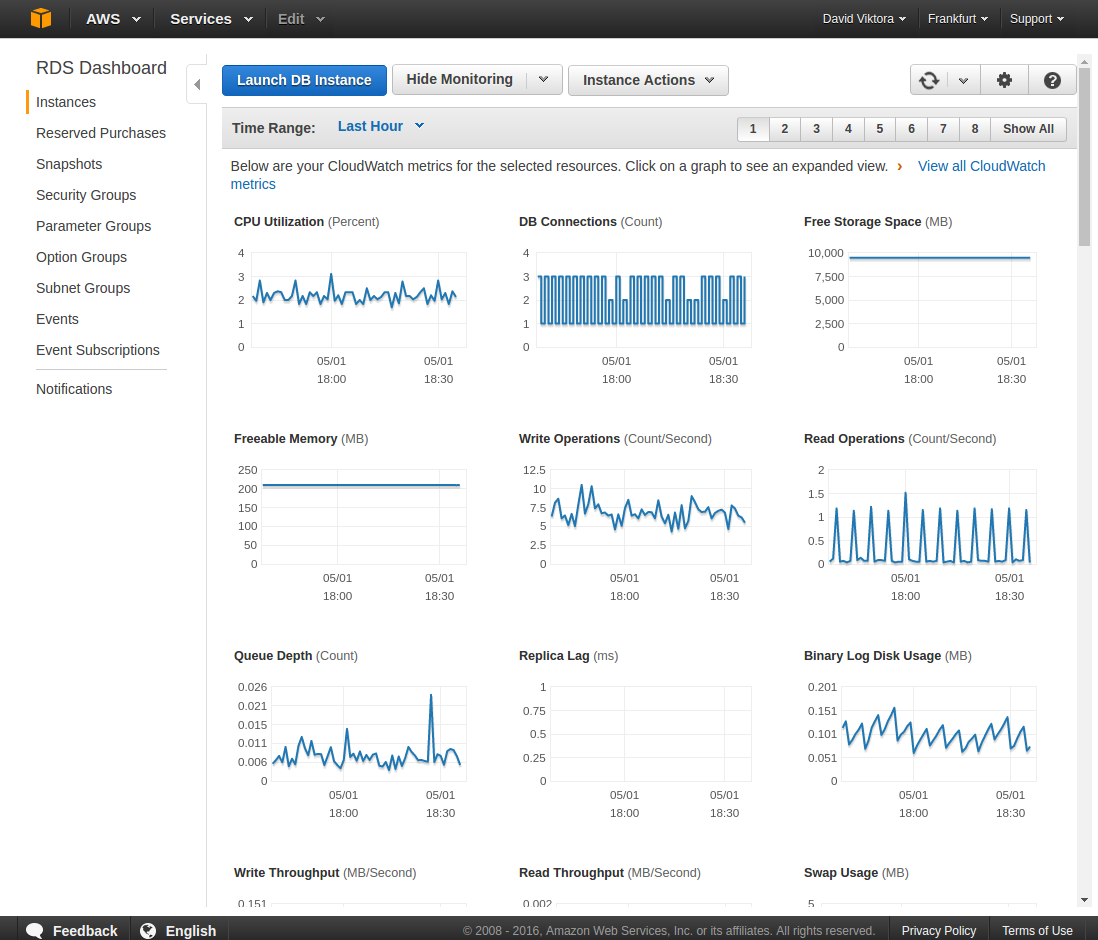
\includegraphics[width=1\textwidth]{images/aws-monitoring.png}
   	\caption{Monitoring databáze v Amazon RDS}
   	\label{fig:aws_monitoring}
\end{figure}
	
\subsection{Agregace dat v čase}
\label{agregace-dat}
	Jedním z funkčních požadavků této práce je agregace statistických dat dle času. Té je možné dosáhnout například pomocí CRONu nebo přímo na úrovni databáze pomocí Event Scheduleru. 
	
	CRON je unixový systémový démon zajišťující provádění uživatelem definovaných příkazů v daném čase. Stačilo by tedy napsat jednoduchý script, který by se připojil k databázi a provedl sloučení dat. Tento skript by pak byl pomocí CRONu pravidelně spouštěn. Protože byl pro nasazení databáze zvolen Amazon RDS, nemáme přístup k celému systému na kterém databáze běží, ale pouze k samotné databázi. CRON proto není vhodným řešením. 
	
	Event Scheduler poskytovaný přímo jako součást MySQL je naopak řešením ideálním. Jeho využití je oproti CRONu omezenější, nicméně pro námi požadovanou agregaci dat je jeho funkcionalita postačující. Půjde navíc o čistší řešení, protože bude operace modifikující databázi řešena přímo na její úrovni. 
	
	Příkaz pro vytvoření eventu agregujího data z tabulky \textit{stats\_general\_3s} do tabulky \textit{stats\_general\_10m }pak vypadá takto:

\begin{figure}
\begin{lstlisting}[language=json,firstnumber=1]
CREATE EVENT `stats_general_3s_to_10m` 
ON SCHEDULE EVERY 10 MINUTE STARTS '2016-01-01 00:01:00' 
ON COMPLETION NOT PRESERVE ENABLE COMMENT 
	'Aggregate general stats 3s -> 10m' 
DO BEGIN 
	INSERT INTO stats_general_10m (tweets_total, 
		tweets_english, wishes_total, 
		sentiment_average) 
	SELECT SUM(tweets_total), SUM(tweets_english), 
		SUM(wishes_total), AVG(sentiment_average) 
	FROM stats_general_3s 
	WHERE datetime > timestamp(utc_timestamp() 
		- interval 10 minute); 
END;
\end{lstlisting}
\caption{MySQL Event provádějící agregaci dat}
\label{fig:mysql-event-agr}
\end{figure} 

Tento příkaz však provádí pouze slučování dat. Pro mazání dat starých bylo potřeba vytvořit další event. Ten zajišťuje mazání dat starších než 30 minut v tabulce stats\_general\_3s:

\begin{figure}
\begin{lstlisting}[language=json,firstnumber=1]
CREATE EVENT `stats_general_3s_clean` 
ON SCHEDULE EVERY 10 MINUTE STARTS '2016-01-01 00:00:00' 
ON COMPLETION NOT PRESERVE ENABLE COMMENT 'Clean old data 
FROM stats_general_3s' DO 
	DELETE FROM stats_general_3s
	WHERE datetime < timestamp(utc_timestamp() 
		- interval 1 hour) */ ;;
\end{lstlisting}
\caption{MySQL provádějící smazání starých dat}
\label{fig:mysql-event-del}
\end{figure} 

\section{API webserver}
\subsection{Výběr technologií}
	Frameworky umožňující implementaci RESTového API existují pro víceméně všechny rozšířené programovací jazyky, některé z nich se však pro tyto účely hodí víc než jiné. Velice oblíbeným je například jazyk Python, který jsem především z důvodů jako jsou skvělá přehlednost kódu a rozsáhlá komunita zvolil i já. Z konkrétních frameworků jsem se poté rozhodoval především mezi minimalistickým Flaskem a komplexnějším Djangem. 
	
	Oba tyto frameworky mají kvalitní dokumentaci a stojí za nimi rozsáhlá komunita. Django je ale určený především pro tvorbu komplexních webových aplikací, kdežto Flask je označován za tzv. micro-framework. Poskytuje tedy jen základní funkcionality, které je možné rozšířit instalací dalších pluginů. Protože cílem je vytvoření pouze RESTového API, je Flask ideálním nástrojem bez pro tento projekt zbytečných funkcí. 
	
\noindent Při implementaci bylo použito několik pluginů pro Flask:
	
\begin{itemize}
\item \textbf{flask-sqlalchemy} - SQLAlchemy je asi nejrozšířenějším ORM\footnote{XXXX} pro Python. Tento plugin integruje jeho funkcionality do frameworku Flask. Umožňuje tedy namapování jednotlivých tabulek databáze na třídy, se kterými je v programu možno jednoduše pracovat místo manuálního vytváření SQL dotazů. 
\item \textbf{flask-restless} - Tento plugin dále využívá SQLAlchemy a umožňuje především automatické vytváření API endpointů na základě definovaných databázových modelů. 
\item \textbf{flask-testing} - Flask-testing je plugin použitý pro testování API endpointů. Tomu se podrobněji věnuji v sekci \ref{api-testing}.
\end{itemize}

\subsection{Ukázky implementace}
Jednotlivé tabulky databáze jsou tedy pomocí ORM SQLAlchemy namapovány na třídy reprezentující objekty jako \textit{user} nebo \textit{tweetWish}. Příklad takového namapování tabulky user ukazuje zdrojový kód \ref{fig:user-orm}. Metodu \textit{json\_dump} bylo nutné naimplementovat pro všechny třídy. Ne všechny atributy jsou totiž serializovatelné a není je tak možné automaticky převádět na JSON. 

\begin{figure}
\begin{lstlisting}[language=json,firstnumber=1][h]
class User(db.Model):
	def __init__(self, id, username, profile_picture_url):
		self.id = id
		self.username = username
		self.profile_picture_url = profile_picture_url

	__tablename__ = 'users'
	id = db.Column(db.BigInteger, primary_key=True)
	username = db.Column(db.String(140))
	profile_picture_url = db.Column(db.Text)
	wishes = relationship("TweetWish",
							back_populates="user")
	mentioned_in = relationship("TweetWish",
    							 secondary=tweet_mentions_user,
								 lazy='dynamic',
								 back_populates="mentioned_users")

	def json_dump(self):
		return dict(id=str(self.id),
					username=self.username,
					profile_picture_url=self.profile_picture_url)
\end{lstlisting}
\caption{Ukázka použití ORM SQLAlchemy}
\label{fig:user-orm}
\end{figure} 

Po namapování všech potřebných tabulek již můžeme v rámci programu pracovat s definovanými třídami. To platí i při vytváření konkrétních endpointů jak ukazuje zdrojový kód \ref{fig:user-view}. Po definování konkrétní cesty, v tomto případě \textit{/user/<user\_id>/}, již dochází jen ke kontrole počtu zadaných argumentů. Poté je jednoduše vrácen JSON obsahující údaje uživatele s daným ID nebo v případě neexistujícího uživatele HTTP status 404. 

Obdobným způsobem jsou implementovány i další endpointy. Zajímavá je také nutnost přidání tzv. CORS hlaviček ke všem odpovědím. CORS neboli Cross Origin Resource Sharing je mechanismus umožňující webům získávání zdrojů z jiných domén. To je ale standardně z bezpečnostních důvodů zakázáno. 

\begin{figure}
\begin{lstlisting}[language=json,firstnumber=1][h]
# return user with specified id
@app.route('/user/<user_id>/', methods=['GET'])
def user(user_id):
	if len(request.args) != 0:
		raise ProcessingException(
				description='Invalid argument provided',
				code=400)

	user = User.query\
		.get_or_404(user_id)
	return jsonify(user.json_dump())
\end{lstlisting}
\caption{Ukázka implementace konkrétního API endpointu}
\label{fig:user-view}
\end{figure} 

\subsection{Nasazení}
Stejně jako v případě databáze, i pro webserver byly využity cloudové služby. Volba probíhala především mezi již probíraným Amazon AWS nebo službou zvanou Heroku. Pro webserver by v případě Amazon AWS bylo nutno použít službu EC2, tedy virtuální server. EC2 je příkladem v kapitole \ref{amazon-aws} již popisovaného modelu IaaS. Heroku je však příkladem platformy (PaaS) umožňující mimojiné i jednoduché spouštění aplikací psaných v Pythonu. Protože v případě Heroku odpadá nutnost administrace linuxového serveru a první nasazení aplikace je na něm otázkou několika minut, je pro námi požadovaný jednoduchý webserver skvělou volbou. 

\subsubsection{Heroku}
Po vytvoření účtu na Heroku je potřeba stáhnout si tzv. Heroku Toolbelt. Jedná se o CLI\footnote{CLI} nástroj sloužící právě ke správě a monitorování aplikací běžících v Heroku cloudu. Při vytváření nové aplikace si uživatel stejně jako v případě Amazon AWS nejdříve zvolí variantu služby na základě jeho hardwarových a jiných požadavků. 

Konkrétní způsob nasazení aplikace se pak mírně liší pro každý z podporovaných jazyků, kterých je momentálně 8. V případě pythonu je nejdříve nutné vytvořit několik souborů:

\begin{itemize}
\item \textbf{requirements.txt} - seznam požadovaných knihoven pro Python vygenerovaný pomocí nástroje pip\footnote{pip}, konkrétně příkazem \textit{pip freeze}.
\item \textbf{Procfile} - soubor určující jak a který soubor spustit po nahrání aplikace na Heroku
\item \textbf{runtime.txt} - určení verze pythonu použité pro spuštění aplikace
\end{itemize}

Nahrání aplikace na Heroku může probíhat několika způsoby, tím základním je ale pooužití GITu. Samotným vytvoření aplikace pomocí Heroku Toolbeltu dojde k přidání remote repozitáře. Do něj poté stačí nahrát změny v repozitáři a Heroku již v případě nenalezení problémů zařídí spuštění aplikace. 

Protože k verzování této práce byl použit jeden společný repozitář namísto oddělených repozitářů pro každou komponentu, nastal samozřejmě problém s nahráním pouze adresáře obsahujícího soubory pro webserver. I toho je ale pomocí GITu možné dosáhnout, použit byl příkaz \textit{git subtree}:


\begin{lstlisting}[language=json,firstnumber=1][ht]
git push heroku_remote `git subtree split --prefix flask_api master`:master --force
\end{lstlisting}



\section{Webová aplikace}
	Jako součást této práce byla pro prezentaci výsledků analýzy vytvořena i webová apliace využívající API popsané v předchozí kapitole. Protože web není součástí zadání této práce, budu se mu podrobněji věnovat pouze z hlediska testování API v kapitole \ref{testovani}. Ukázky této aplikace jsou pak k nalezení v příloze \ref{appendix-web}.  
	
	Webová aplikace je napsána pomocí jazyků HTML, CSS a JavaScript, použity byly i komponenty frameworku Bootstrap. K nasazení byl použit Amazon AWS, konkrétně služby Amazon S3 pro hostování dat a Amazon Route 53 pro nastavení vlastního doménového jména. 


\chapter{Testování}
\label{testovani}
Testovování je důležitou součástí vývoje každého software a jinak tomu není ani v případě systému implementovaného v rámci této práce. Kromě manuálního testování prováděného během vývoje systému byly implementovány i automatické testy poskytovaného API. Pro prezentaci výsledků analýzy a zároveň pro otestování celého systému byl vytvořen také web zobrazující informace o analyzovaných přáních. 


\section{Test API endpointů}
\label{api-testing}
Při testování implementovaného API bylo použito rozšíření pro framework Flask zvané Flask-testing. To využívá knihovnu unittest, která je součástí standardní Python knihovny, a přidává několik funkcionalit zjednodušujících použití v rámci Flasku. 

Po vytvoření třídy dědící od třídy TestCase je nejrpve nutné vytvořit několik metod:

\begin{itemize}
\item \textbf{create\_app} - jde o metodu volanou ještě před spuštěním prvního testu. Lze v ním například změnit konfigurační soubor a použít díky tomu testovací instanci databáze místo té produkční. 
\item \textbf{setUp} - tato metoda je spuštěna před každým jednotlivým testem. Jejím hlavním úkolem je naplnění databáze daty, která budou následně využita při testování. 
\item \textbf{tearDown} - metoda tearDown je naopak spouštěna na konci každého testu. V ní je obvykle databáze naopak přemazána. 
\end{itemize}

Poté již stačí vytvořit jednotlivé testy. Za ty se automaticky považují všechny metody, jejichž název začíná slovem test. Ukázku testu zaměřeného na endpoint /user/<user\_id> zobrazuje zdrojový kód \ref{user-test}. U všech endpointů je testován především návratový kód, v některých případech i konkrétní odpověď webserveru. 


\lstset{captionpos=b, caption={Descriptive Caption Text},label=user-test}
\begin{lstlisting}[language=json,firstnumber=1][ht]
def test_user_detail(self):
	response = self.client.get('/user/123/', query_string={})
	assert response.status_code == 200
	user = {'username': 'Jack', 'id': '123', 'profile_picture_url': 'http://profile.picture.url'}
	self.assertEqual(response.json, user)
\end{lstlisting}


\section{Web prezentující výsledky analýzy}
Vytvořenou webovou stránku je možné nalézt na adrese http://tweetwishes.com, pro jeho plnou funkcionalitu však musí být spuštěn i samotný systém pro analýzu tweetů. Na webu jsou totiž v reálném čase zobrazována nová přání, statistiky a další údaje. Obrázky webu jsou k dispozici v příloze \ref{appendix-web}. 


\chapter{Zhodnocení výsledků}
\label{zhodnoceni}
Implementovaný systém dle požadavků provádí analýzu příspěvků publikovaných na Twitteru. Přestože původní plán rychlosti zpracování těchto příspěvků počítal s kratší doubou analýzy, její výsledky jsou dostupné na webu již během několika desítek sekund po publikování tweetů. Toto zpoždění je způsobeno slabým výpočetním výkonem a overheadem potřebným pro inicializaci Sparku a distribuci operací a dat. 

Prováděná analýza vedla k zajímavým výsledkům. Jak ukazuje graf na obrázku \ref{fig:sentiment-graph}, výrazně převažují negativní přání nad těmi pozitivními. Monitorováním nejpoužívanějších hashtagů bylo například možné sledovat vývoj amerických prezidentských voleb, velice aktivní byly také uživatelé z Filipín. I ti vyjadřovali svá přání týkající se voleb nového filipínského prezidenta. Kromě politických témat se v přáních často objevovala sportovní témata či příspěvky týkající se hudebních a filmových hvězd. 
\begin{figure}[h]
   	\centering
   	
\includegraphics[width=1\textwidth]{images/cvut-logo-bw.pdf}
   	\caption{Zde bude graf vývoje sentimentu}
   	\label{fig:sentiment-graph}
\end{figure}

\section{Využití systému}
V současném stavu je implementovaný systém určen především pro pobavení a prezentaci použitých technologií. Nabízí se však několik možných využítí, kterých by bylo možné dosáhnout jen drobnými úpravami tohoto systému. 

Díky prováděné analýze sentimentu by mohlo jít obecně o úlohy zabývající se tzv. opinion miningem - díky analýze sentimentu příspěvků obsahujících dané výrazy či hashtagy by bylo možné například provádět předvolební průzkumy, hodnotit úspěšnost reklamní kampaně či určovat oblíbenost zvolených produktů a značek. 


\section{Možná budoucí vylepšení}
Jedním z hlavních vylepšení systému by bylo bezesporu jeho nasazení na počítačový cluster. K tomu je celý systém připravený a díky dostupnému výkonu by stálo za zvážení zažádat o přístup k veškerým příspěvkům z Twitteru pomocí služby Gnip popsané v sekci \ref{twitter-api}. 

Nabízí se i několik funkčních vylepšení celého systému. Jedním z nich jeho jeho zobecnění, díky kterému by jeho využití nebylo omezeno na analýzů přání uživatelů, ale bylo by ho možné využívat například i pro výše zmíněné účely. Filtrované výrazy by byly zadány například do konfiguračního souboru. Až na přejmenování tabulek a proměnných by jiné výraznější zásahy do systému nebyly nutné. 

Systém by také jistě bylo možné optimalizovat a snížit tak rychlost analýzy tweetů. Jednou z možností by bylo využití noSQL databáze a kompletní změna způsobu ukládání dat. Práce s relační SQL databází pomocí SparkSQL je totiž v některých směrech omezující a některé operace mohou dobu zpracování nežádoucím způsobem zvyšovat. 

Zajímavé by bylo také rozšíření systému o další metody z oblasti text miningu a zpracování řeči, jejichž použití by v kontextu sociální sítě Twitter dávalo smysl. 

\begin{conclusion}
	Zaver
\end{conclusion}



\begin{thebibliography}{1}

\bibitem{bbc-bigdata} WALL, Matthew. Big Data: Are you ready for blast-off? In: BBC News [online]. 2014 [cit. 2016-04-10]. Dostupné z: http://www.bbc.com/news/business-26383058

\bibitem{internet-live-stats} Internet Users. Internet Live Stats: Internet Usage \& Social Media Statistics [online]. [cit. 2016-04-10]. Dostupné z: http://www.internetlivestats.com/internet-users/

\bibitem{bigdata-iot} Why Big Data And The Internet of Things Are A Perfect Match. In: Datamation: IT Management, IT Salary, Cloud Computing, Open Source, Virtualization, Apps. [online]. [cit. 2016-04-10]. Dostupné z: http://www.datamation.com/applications/why-big-data-and-the-internet-of-things-are-a-perfect-match.html

\bibitem{webopedia-bigdata} What is big data? Webopedia: Online Tech Dictionary for IT Professionals [online]. [cit. 2016-04-11]. Dostupné z: http://www.webopedia.com/TERM/B/big\_data.html

\bibitem{dp-customer-inteligence} TŘÍSKA, Martin. Customer Intelligence v kontextu Big Data. Praha, 2013. Diplomová práce. České vysoké učení technické v Praze. Vedoucí práce Tomáš Bruckner.

\bibitem{structured-unstructured}Structured vs. Unstructured Data: The Rise of Data Anarchy. In: Data Science Central [online]. [cit. 2016-04-11]. Dostupné z: http://www.datasciencecentral.com/profiles/blogs/structured-vs-unstructured-data-the-rise-of-data-anarchy

\bibitem{stock-stanford}MITTAL, Anshul a Arpit GOEL. Stock Prediction Using Twitter Sentiment Analysis. 2012. Dostupné také z: http://cs229.stanford.edu/proj2011/GoelMittal-StockMarketPredictionUsingTwitterSentimentAnalysis.pdf. Standford University.

\bibitem{mapreduce-google}DEAN, Jeffrey a Sanjay GHEMAWAT. MapReduce: simplified data processing on large clusters. Google Inc., 2004.

\bibitem{mapreduce-description}What is MapReduce. IBM [online]. [cit. 2016-04-11]. Dostupné z: https://www-01.ibm.com/software/data/infosphere/hadoop/mapreduce/

\bibitem{mapreduce-img}MapReduce introduction. Computer Science [online]. [cit. 2016-04-16]. Dostupné z: http://www.cs.uml.edu/~jlu1/doc/source/report/MapReduce.html

\bibitem{hadoop-history}The history of Hadoop: From 4 nodes to the future of data. In: Gigaom: The industry leader in emerging technology research [online]. [cit. 2016-04-17]. Dostupné z: https://gigaom.com/2013/03/04/the-history-of-hadoop-from-4-nodes-to-the-future-of-data/

\bibitem{spark-home}Apache Spark: Ligthtning-Fast Cluster Computing [online]. [cit. 2016-04-17]. Dostupné z: http://spark.apache.org/

\bibitem{hadoop-home}Welcome to Apache Hadoop! [online]. [cit. 2016-04-17]. Dostupné z: http://hadoop.apache.org/

\bibitem{streaming-benchmark}Benchmarking Streaming Computation Engines at Yahoo!. Yahoo Engineering [online]. [cit. 2016-04-17]. Dostupné z: https://yahooeng.tumblr.com/post/135321837876/benchmarking-streaming-computation-engines-at

\bibitem{flink-future}Fast Big Data: Apache Flink vs Apache Spark for Streaming Data. Analytics, Data Mining, and Data Science [online]. [cit. 2016-04-17]. Dostupné z: http://www.kdnuggets.com/2015/11/fast-big-data-apache-flink-spark-streaming.html

\bibitem{spark-components}The 5-Minute Guide to Understanding the Significance of Apache Spark. Big Data Hadoop Blog | MapR [online]. [cit. 2016-04-17]. Dostupné z: https://www.mapr.com/blog/5-minute-guide-understanding-significance-apache-spark

\bibitem{streaming-guide}Spark Streaming Programming Guide. Overview - Spark 1.6.1 Documentation [online]. [cit. 2016-04-17]. Dostupné z: http://spark.apache.org/docs/latest/streaming-programming-guide.html

\bibitem{so-flink-storm}What is/are the main difference(s) between Flink and Storm? Stack Overflow [online]. [cit. 2016-04-17]. Dostupné z: http://stackoverflow.com/questions/30699119/what-is-are-the-main-differences-between-flink-and-storm

\bibitem{spark-toplevel}The Apache Software Foundation Announces Apache Spark as a Top-Level Project. The Apache Software Foundation [online]. [cit. 2016-04-17]. Dostupné z: https://blogs.apache.org/foundation/entry/the\_apache\_software\_foundation\_announces50

\bibitem{spark-mapreduce-difference}What is the difference between Apache Spark and Apache Hadoop (Map-Reduce) ? Quora [online]. [cit. 2016-04-17]. Dostupné z: https://www.quora.com/What-is-the-difference-between-Apache-Spark-and-Apache-Hadoop-Map-Reduce

\bibitem{google-pagerank}Getting started with Apache Spark GraphX – Part 1. PhData [online]. [cit. 2016-04-17]. Dostupné z: https://phdata.io/getting-started-with-apache-spark-graphx-part-1/

\bibitem{twitter-stats}By The Numbers: 170+ Amazing Twitter Statistics. DMR [online]. [cit. 2016-04-19]. Dostupné z: http://expandedramblings.com/index.php/march-2013-by-the-numbers-a-few-amazing-twitter-stats/

\bibitem{twitter-stats-2}Twitter Usage Statistics. Internet Live Stats: Internet Usage \& Social Media Statistics [online]. [cit. 2016-04-19]. Dostupné z: http://www.internetlivestats.com/twitter-statistics/

\bibitem{twitter-140}Twitter Basics: Why 140-Characters, And How to Write More. Social Times: Covering the world of social media [online]. [cit. 2016-04-19]. Dostupné z: http://www.adweek.com/socialtimes/twitter-basics-why-140-characters-and-how-to-write-more/442608

\bibitem{twitter-api}GET statuses/sample. Twitter Developers [online]. [cit. 2016-04-20]. Dostupné z: https://dev.twitter.com/streaming/reference/get/statuses/sample

\bibitem{twitter-rest-stream}The Streaming APIs Overview. Twitter Developers [online]. [cit. 2016-04-20]. Dostupné z: https://dev.twitter.com/streaming/overview

\bibitem{twitter4j}Twitter4J - A Java library for the Twitter API [online]. [cit. 2016-04-20]. Dostupné z: http://twitter4j.org/en/index.html

\bibitem{gnip}Gnip: Unleash the Power of Social Media [online]. [cit. 2016-04-20]. Dostupné z: https://gnip.com/

\bibitem{nosql-dbs}NOSQL Databases [online]. [cit. 2016-04-26]. Dostupné z: http://nosql-database.org/

  
\end{thebibliography}



\appendix

\chapter{Definice API endpointů}
\label{appendix-api}
\begin{table}[h]
\begin{tabular}{llllr}
\rowcolor[HTML]{EFEFEF}
\large \textbf{/wish/}        &         &                 &        & \multicolumn{1}{l}{}                \\
\rowcolor[HTML]{EFEFEF}
\textbf{GET}          &         &                 &        & Seznam přání                        \\
\multicolumn{5}{l}{\parbox[t]{12.8cm}{Bez použití následujích parametrů vrátí všechna přání za posledních 10 minut. Při použití \textit{count} jsou ignorovány parametry  \textit{from} a \textit{to}.}  } \\
\textbf{from}         &         & timestamp       &        & od včetně                           \\
\textbf{to}           &         & timestamp       &        & do vyjímaje                         \\
\textbf{count}        &         & integer         &        & omezení počtu vrácených přání      \\
 & & & & \\
 Příklad odpovědi:
\end{tabular}
\end{table}

\begin{lstlisting}[language=json,firstnumber=1]
 {
  "wishes": [
    {
      "author": {
        "id": 2745306105,
        "profile_picture_url": "http://pbs.twimg.com/..",
        "username": "moley Jem"
      },
      "created_at": "2016-04-25 20:13:11",
      "id": 724692755319021569,
      "is_retweet": false,
      "retweet_tweet_id": 724692755319021569,
      "sentiment": 1.0,
      "tweet_text": "I just wish...that's all"
    },
    ...
    ]
 }
\end{lstlisting}[language=json,firstnumber=1]


\begin{table}[h]
\begin{tabular}{llllr}
\rowcolor[HTML]{EFEFEF}
\large \textbf{/wish/\{wish\_id\}}        &         &                 &        & \multicolumn{1}{l}{}                \\
\rowcolor[HTML]{EFEFEF}
\textbf{GET}          &         &                 &        & Konkrétní přání                        \\
\multicolumn{5}{l}{\parbox[t]{12.8cm}{Vrací stejné údaje jako \textit{/wish/}, ale pouze pro konkrétní přání s daným \textit{wish\_id}.}  } \\  
 & & & & \\
 Příklad odpovědi:
\end{tabular}
\end{table}
 
\begin{lstlisting}[language=json,firstnumber=1]
{
  "author": {
    "id": 19748673,
    "profile_picture_url": "http://pbs.twimg.com/pro...",
    "username": "DJ Romeo Reyes"
  },
  "created_at": "2016-04-25 20:12:44",
  "id": 724692642039111680,
  "is_retweet": false,
  "retweet_tweet_id": 724692642039111680,
  "sentiment": 2.0,
  "tweet_text": "I hope the Blazers take the series to..."
 }
\end{lstlisting} 

\begin{table}[h]
\begin{tabular}{llllr}
\rowcolor[HTML]{EFEFEF}
\large \textbf{/wish/\{wish\_id\}/mentions}        &         &                 &        & \multicolumn{1}{l}{}                \\
\rowcolor[HTML]{EFEFEF}
\textbf{GET}          &         &                 &        & Uživatelé zmíněný v přání                        \\
\multicolumn{5}{l}{\parbox[t]{12.8cm}{Vrací seznam uživatelů zmíněných v přání s daným \textit{wish\_id}.}  } \\    
 & & & & \\
 Příklad odpovědi:
\end{tabular}
\end{table}

\begin{lstlisting}[language=json,firstnumber=1]
 {
  "mentioned_users": [
    {
      "id": 389507955,
      "profile_picture_url": "",
      "username": "EJ Gomez"
    },
    ...
  ]
 }
\end{lstlisting} 

\begin{table}[h]
\begin{tabular}{llllr}
\rowcolor[HTML]{EFEFEF}
\large \textbf{/wish/\{wish\_id\}/hashtags}        &         &                 &        & \multicolumn{1}{l}{}                \\
\rowcolor[HTML]{EFEFEF}
\textbf{GET}          &         &                 &        & Hashtagy použité v přání                        \\
\multicolumn{5}{l}{\parbox[t]{12.8cm}{Vrací seznam hashtagů použitch v přání s daným \textit{wish\_id}.}  } \\   
 & & & & \\
 Příklad odpovědi: 
\end{tabular}
\end{table}

\begin{lstlisting}
TODO
\end{lstlisting} 

\begin{table}[h]
\begin{tabular}{llllr}
\rowcolor[HTML]{EFEFEF}
\large \textbf{/user/}        &         &                 &        & \multicolumn{1}{l}{}                \\
\rowcolor[HTML]{EFEFEF}
\textbf{GET}          &         &                 &        & Seznam uživatelů                        \\
\multicolumn{5}{l}{\parbox[t]{12.8cm}{Vrací seznam všech uživatelů, tedy autorů přání nebo uživatelů zmíněných v některém z nich. }  } \\   
 & & & & \\
 Příklad odpovědi:
\end{tabular}
\end{table}

\begin{lstlisting}[language=json,firstnumber=1]
 {
  "users": [
    {
      "id": 12,
      "profile_picture_url": "",
      "username": "Jack"
    },
    ...
    ]
 }
\end{lstlisting} 

\begin{table}[h]
\begin{tabular}{llllr}
\rowcolor[HTML]{EFEFEF}
\large \textbf{/user/\{user\_id\}}        &         &                 &        & \multicolumn{1}{l}{}                \\
\rowcolor[HTML]{EFEFEF}
\textbf{GET}          &         &                 &        & Konkrétní uživatel                        \\
\multicolumn{5}{l}{\parbox[t]{12.8cm}{Vrací údaje o konkrétním uživateli s daným \textit{user\_id}. }  } \\  
 & & & & \\
 Příklad odpovědi:
\end{tabular}
\end{table}

\begin{lstlisting}[language=json,firstnumber=1]
 {
  "id": 12,
  "profile_picture_url": "",
  "username": "Jack"
 }
\end{lstlisting} 

\begin{table}[h]
\begin{tabular}{llllr}
\rowcolor[HTML]{EFEFEF}
\large \textbf{/user/\{user\_id\}/wishes}        &         &                 &        & \multicolumn{1}{l}{}                \\
\rowcolor[HTML]{EFEFEF}
\textbf{GET}          &         &                 &        & Přání daného uživatele                        \\
\multicolumn{5}{l}{\parbox[t]{12.8cm}{Vrací seznam přání uživatele s daným \textit{user\_id}. }  } \\  
 & & & & \\
 Příklad odpovědi: viz \textit{/wish/\{wish\_id\}}
\end{tabular}
\end{table}

\begin{table}[h]
\begin{tabular}{llllr}
\rowcolor[HTML]{EFEFEF}
\large \textbf{/user/\{user\_id\}/mentioned\_in}        &         &                 &        & \multicolumn{1}{l}{}                \\
\rowcolor[HTML]{EFEFEF}
\textbf{GET}          &         &                 &        & Zmínění daného uživatele                        \\
\multicolumn{5}{l}{\parbox[t]{12.8cm}{Vrací seznam přání, ve kterých byl uživatel s daným \textit{user\_id} zmíněn. }  } \\  
 & & & & \\
 Příklad odpovědi: viz \textit{/wish/\{wish\_id\}}
\end{tabular}
\end{table}


\begin{table}[h]
\begin{tabular}{llllr}
\rowcolor[HTML]{EFEFEF}
\large \textbf{/hashtag/\{hashtag\}/wishes}        &         &                 &        & \multicolumn{1}{l}{}                \\
\rowcolor[HTML]{EFEFEF}
\textbf{GET}          &         &                 &        & Přání obsahující daný hashtag                       \\
\multicolumn{5}{l}{\parbox[t]{12.8cm}{Vrací seznam přání, ve kterých byl použit daný \textit{hashtag}. }  } \\  
 & & & & \\
 Příklad odpovědi: viz \textit{/wish/}
\end{tabular}
\end{table}

\begin{table}[h]
\begin{tabular}{llllr}
\rowcolor[HTML]{EFEFEF}
\large \textbf{/stats/mentions}        &         &                 &        & \multicolumn{1}{l}{}                \\
\rowcolor[HTML]{EFEFEF}
\textbf{GET}          &         &                 &        & Seznam zmiňovaných uživatelů                        \\
\multicolumn{5}{l}{\parbox[t]{12.8cm}{Bez použití následujích parametrů vrátí seznam všech zmíněných uživatelů v posledních 10 minutách společně s počtem jejich zmínění. \\ Výsledky jsou řazeny sestupně dle počtu zmínění v daném intervalu. }  } \\
\textbf{from}         &         & timestamp       &        & od včetně                           \\
\textbf{to}           &         & timestamp       &        & do vyjímaje                         \\
\textbf{count}        &         & integer         &        & omezení počtu vrácených uživatelů     \\ 
 & & & & \\
 Příklad odpovědi:
\end{tabular}
\end{table}

\begin{lstlisting}[float=H][language=json,firstnumber=1]
{
  "popular_users": [
    {
      "mention_count": 5,
      "user": {
        "id": 42562446,
        "profile_picture_url": "",
        "username": "Stephen Curry"
      }
    },
    ...
    ]
 }
\end{lstlisting} 

\begin{table}[h]
\begin{tabular}{llllr}
\rowcolor[HTML]{EFEFEF}
\large \textbf{/stats/hashtags}        &         &                 &        & \multicolumn{1}{l}{}                \\
\rowcolor[HTML]{EFEFEF}
\textbf{GET}          &         &                 &        & Seznam používaných hashtagů                        \\
\multicolumn{5}{l}{\parbox[t]{12.8cm}{Bez použití následujích parametrů vrátí seznam všech hashtagů použitých v posledních 10 minutách společně s počtem jejich použití. \\ Výsledky jsou řazeny sestupně dle počtu použití v daném intervalu. }  } \\
\textbf{from}         &         & timestamp       &        & od včetně                           \\
\textbf{to}           &         & timestamp       &        & do vyjímaje                         \\
\textbf{count}        &         & integer         &        & omezení počtu vrácených hashtagů     \\
 & & & & \\
 Příklad odpovědi: 
\end{tabular}
\end{table}

\begin{lstlisting}[float=H][language=json,firstnumber=1]
 {
  "popular_hashtags": [
    {
      "count": 3,
      "hashtag": "dubnation"
    },
    ...
    ]
 }
\end{lstlisting} 


\begin{table}[h]
\begin{tabular}{llllr}
\rowcolor[HTML]{EFEFEF}
\large \textbf{/stats/general}        &         &                 &        & \multicolumn{1}{l}{}                \\
\rowcolor[HTML]{EFEFEF}
\textbf{GET}          &         &                 &        & Obecné statistiky                        \\
\multicolumn{5}{l}{\parbox[t]{12.8cm}{Bez použití následujích parametrů vrátí obecné statistiky za posledních 10 minut.  }  } \\
\textbf{from}         &         & timestamp       &        & od včetně                           \\
\textbf{to}           &         & timestamp       &        & do vyjímaje                         \\
\textbf{density}        &         & "3s"/"10m"/"1d"         &        & hustota statistických dat   \\
 & & & & \\
 Příklad odpovědi:   \\
\end{tabular}
\end{table}

\begin{lstlisting}[float=H][language=json,firstnumber=1]
 {
  "stats": [
    {
      "datetime": "2016-04-25 20:43:29",
      "sentiment_average": 2.1570285426245794,
      "tweets_english": 644,
      "tweets_total": 1591,
      "wishes_total": 9
    },
    ...
    ]
 }
\end{lstlisting}

\chapter{Ukázky webové aplikace}
\label{appendix-web}

\chapter{Seznam použitých zkratek}
% \printglossaries
\begin{description}
	\item[Item1] foo
	\item[Item2] bar
\end{description}

\chapter{Obsah přiloženého CD}

%upravte podle skutecnosti

\begin{figure}
	\dirtree{%
		.1 readme.txt\DTcomment{stručný popis obsahu CD}.
		.1 exe\DTcomment{adresář se spustitelnou formou implementace}.
		.1 src.
		.2 impl\DTcomment{zdrojové kódy implementace}.
		.2 thesis\DTcomment{zdrojová forma práce ve formátu \LaTeX{}}.
		.1 text\DTcomment{text práce}.
		.2 thesis.pdf\DTcomment{text práce ve formátu PDF}.
		.2 thesis.ps\DTcomment{text práce ve formátu PS}.
	}
\end{figure}

\end{document}

\iffalse
\fi
